\chapter{Resultados y visualización}
\label{chap:resultados}

Este capítulo presenta resultados del análisis de los dos CSV recibidos. Las cifras se exportan en \texttt{resultados/metricas.json} y en tablas CSV; las figuras se generan desde el mismo cuaderno. La audiencia es el profesorado de la asignatura y el objetivo es explicar diferencias y coincidencias, no elaborar un catálogo de artistas. Siguiendo la Sesión~6~\cite{sesion6}, se emplean barras para comparar magnitudes, mapas de calor para matrices y dispersión para relaciones entre variables; se evita el doble eje vertical.

\section{Composición y diversidad de etiquetas}

La cobertura de etiquetas por rango está entre el 94\% y el 100\%. La Tabla~\ref{tab:diversidad} separa el tamaño del ranking del número de etiquetas diferentes y de su entropía. Se cuentan asociaciones artista--etiqueta deduplicadas: un artista puede aportar varias, por lo que estas cifras no miden minutos ni reproducciones.

\begin{table}[H]
\centering
\small
\begin{tabular}{llrrrr}
\hline
Usuario & Rango & Artistas & Con etiqueta & Etiquetas & Entropía (bits) \\
\hline
Jorge & 4 semanas & 48 & 48 & 64 & 5,4033 \\
Jorge & 6 meses & 50 & 49 & 64 & 5,3244 \\
Jorge & Varios años & 50 & 49 & 66 & 5,3752 \\
Pablo & 4 semanas & 50 & 47 & 57 & 5,1208 \\
Pablo & 6 meses & 50 & 49 & 60 & 5,1231 \\
Pablo & Varios años & 50 & 50 & 56 & 5,0982 \\
\hline
\end{tabular}
\caption{Diversidad de etiquetas por usuario y rango, calculada sobre artistas con etiquetas.}
\label{tab:diversidad}
\end{table}

En el perfil global de Jorge, \texttt{rock} aparece en 23 artistas distintos, \texttt{alternative} en 16 y \texttt{soundtrack} en 14. En Pablo predominan \texttt{rap} (23), \texttt{rock} (16), \texttt{hip-hop} (15) y \texttt{hip hop} (14). Estas dos últimas grafías se mantienen como etiquetas distintas: no deben sumarse directamente, ya que pueden coexistir en un mismo artista. También sobreviven etiquetas de procedencia como \texttt{spain} o \texttt{japanese}. Por tanto, se analiza una folksonomía musical parcialmente filtrada, no una taxonomía canónica de géneros.

\begin{figure}[H]
\centering
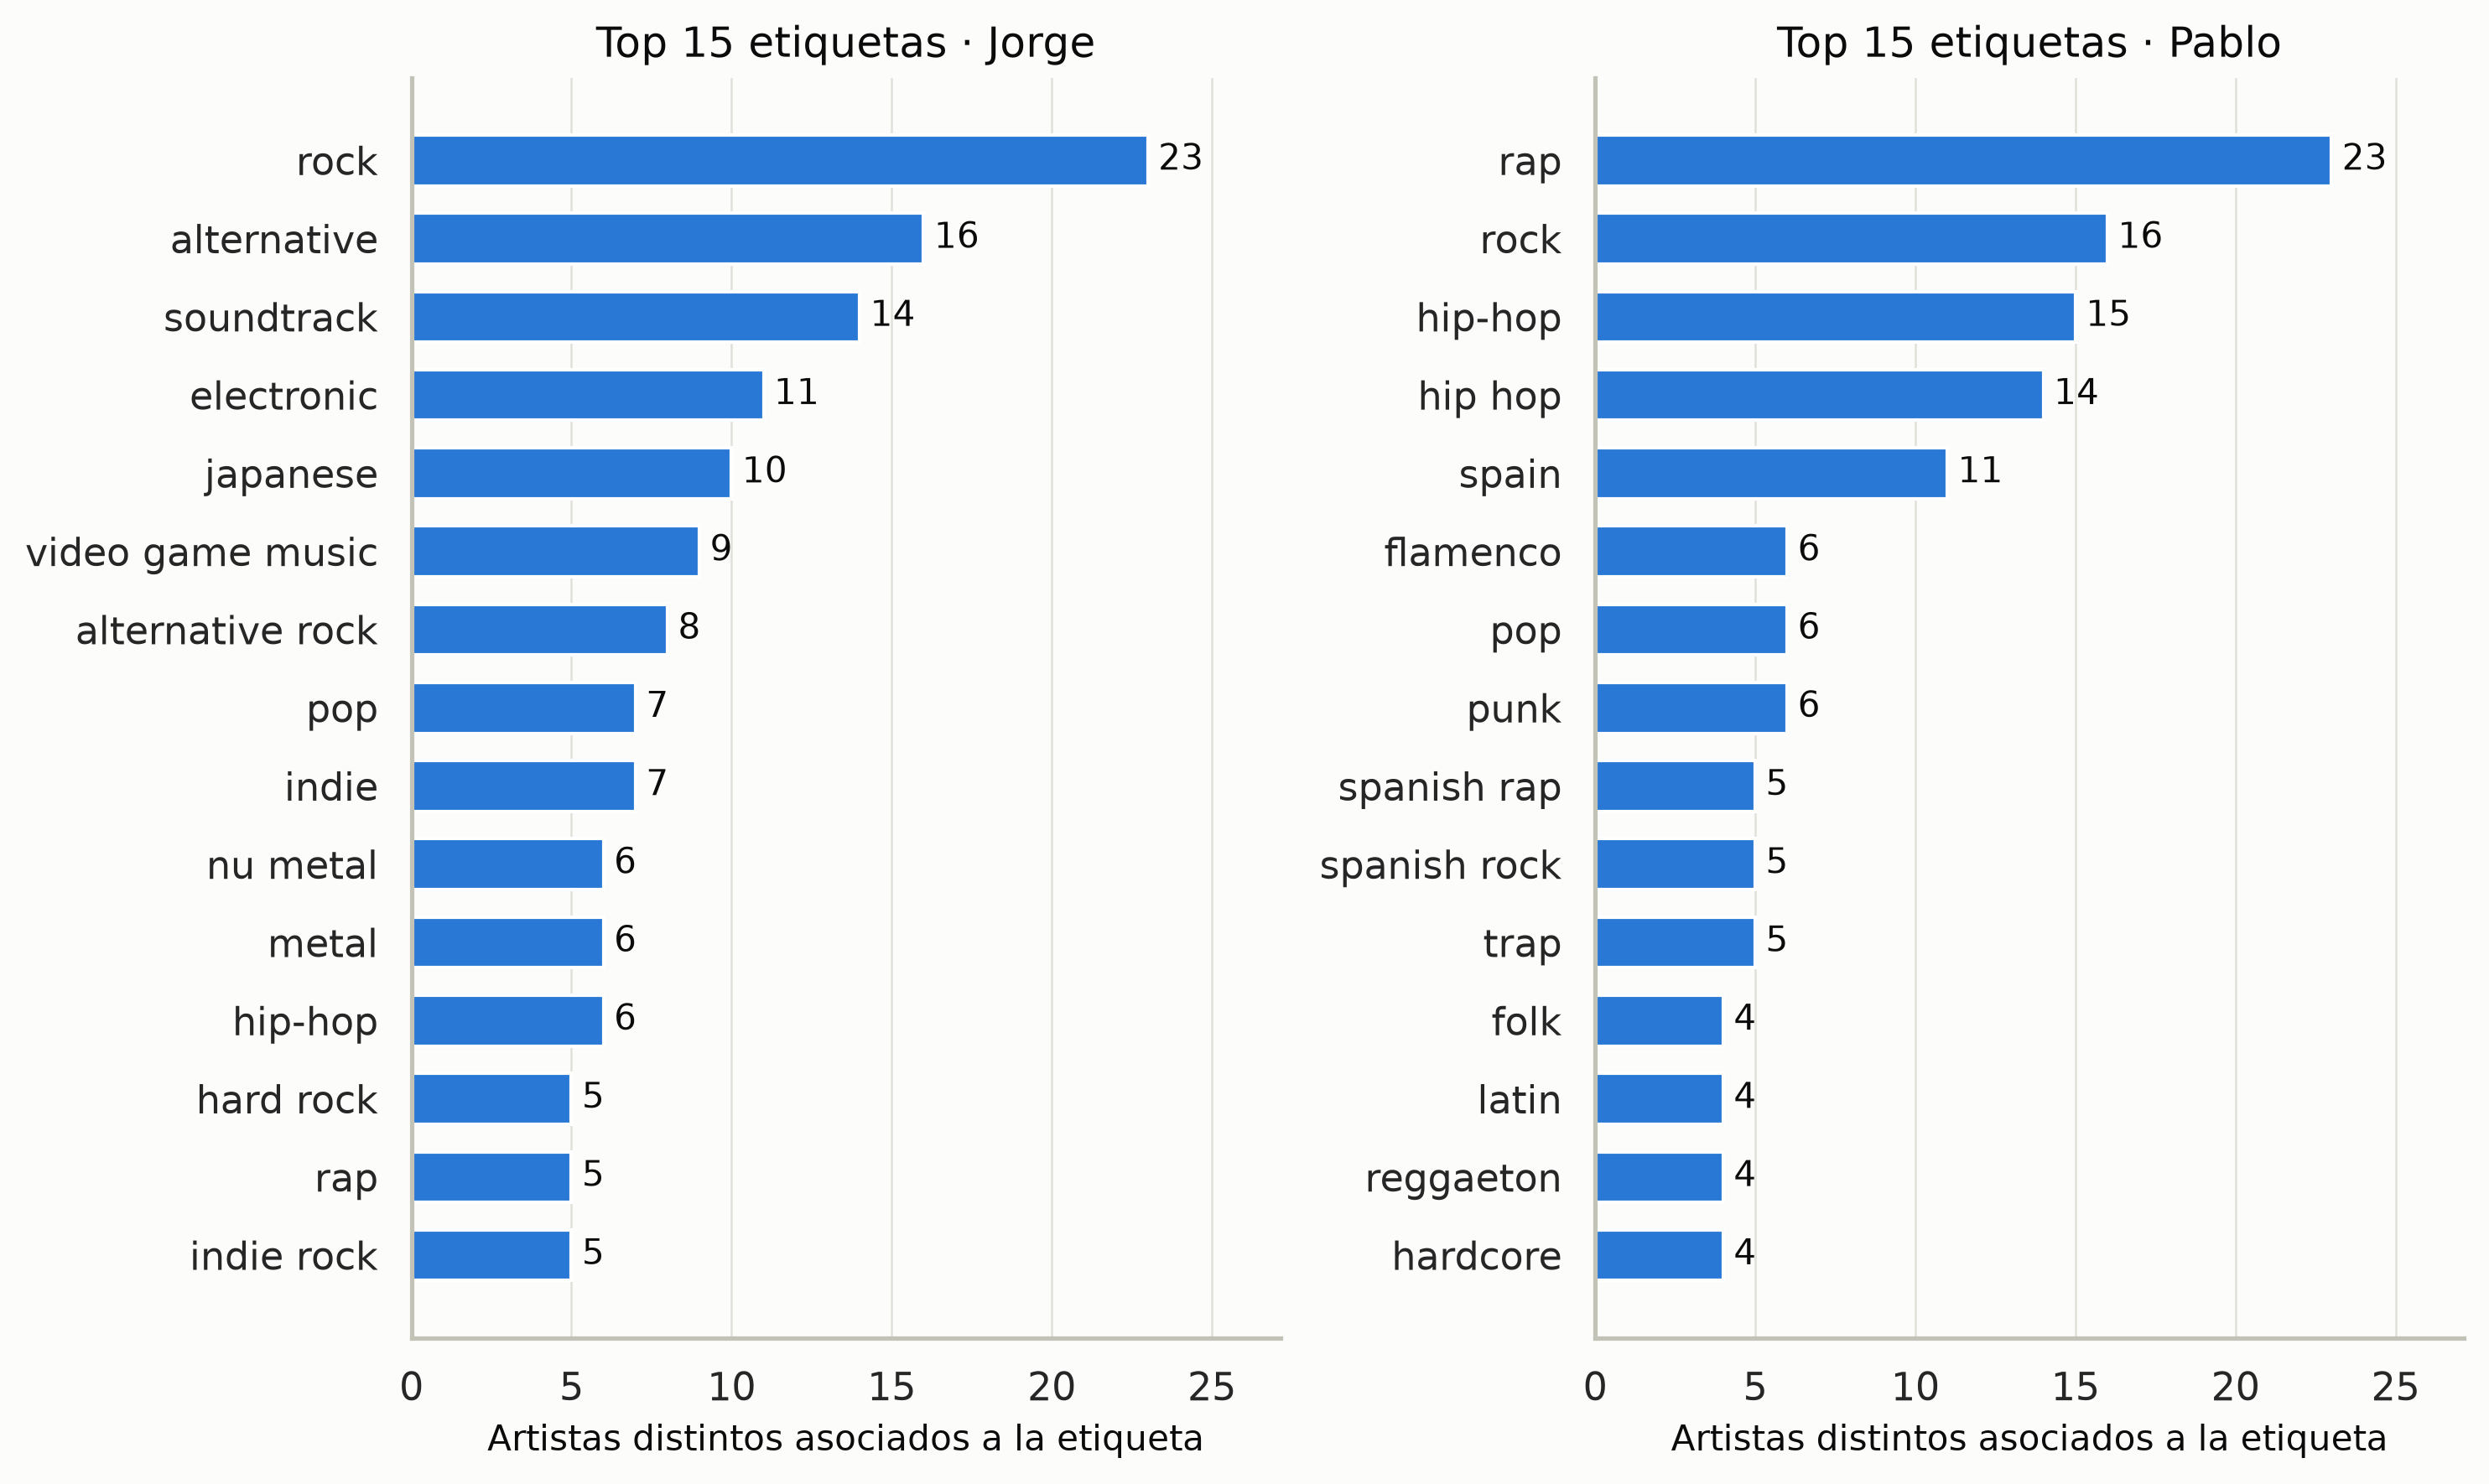
\includegraphics[width=\textwidth]{img/01_top_generos.png}
\caption{Quince etiquetas más frecuentes por usuario. Las barras horizontales facilitan leer nombres largos; ambos paneles comparten escala y muestran el número de artistas distintos.}
\label{fig:top-generos}
\end{figure}

Jorge presenta más etiquetas distintas y mayor entropía en los tres rangos: 5,3244--5,4033 bits frente a 5,0982--5,1231 en Pablo. Esto describe una distribución de etiquetas más dispersa en esta muestra, no demuestra una mayor diversidad musical objetiva: influyen el número de etiquetas por artista, sus sinónimos y la cobertura de Last.fm. La etiqueta más frecuente representa aproximadamente el 9,4--10,2\% de las asociaciones de Jorge y el 12,1--13,5\% de las de Pablo.

\begin{figure}[H]
\centering
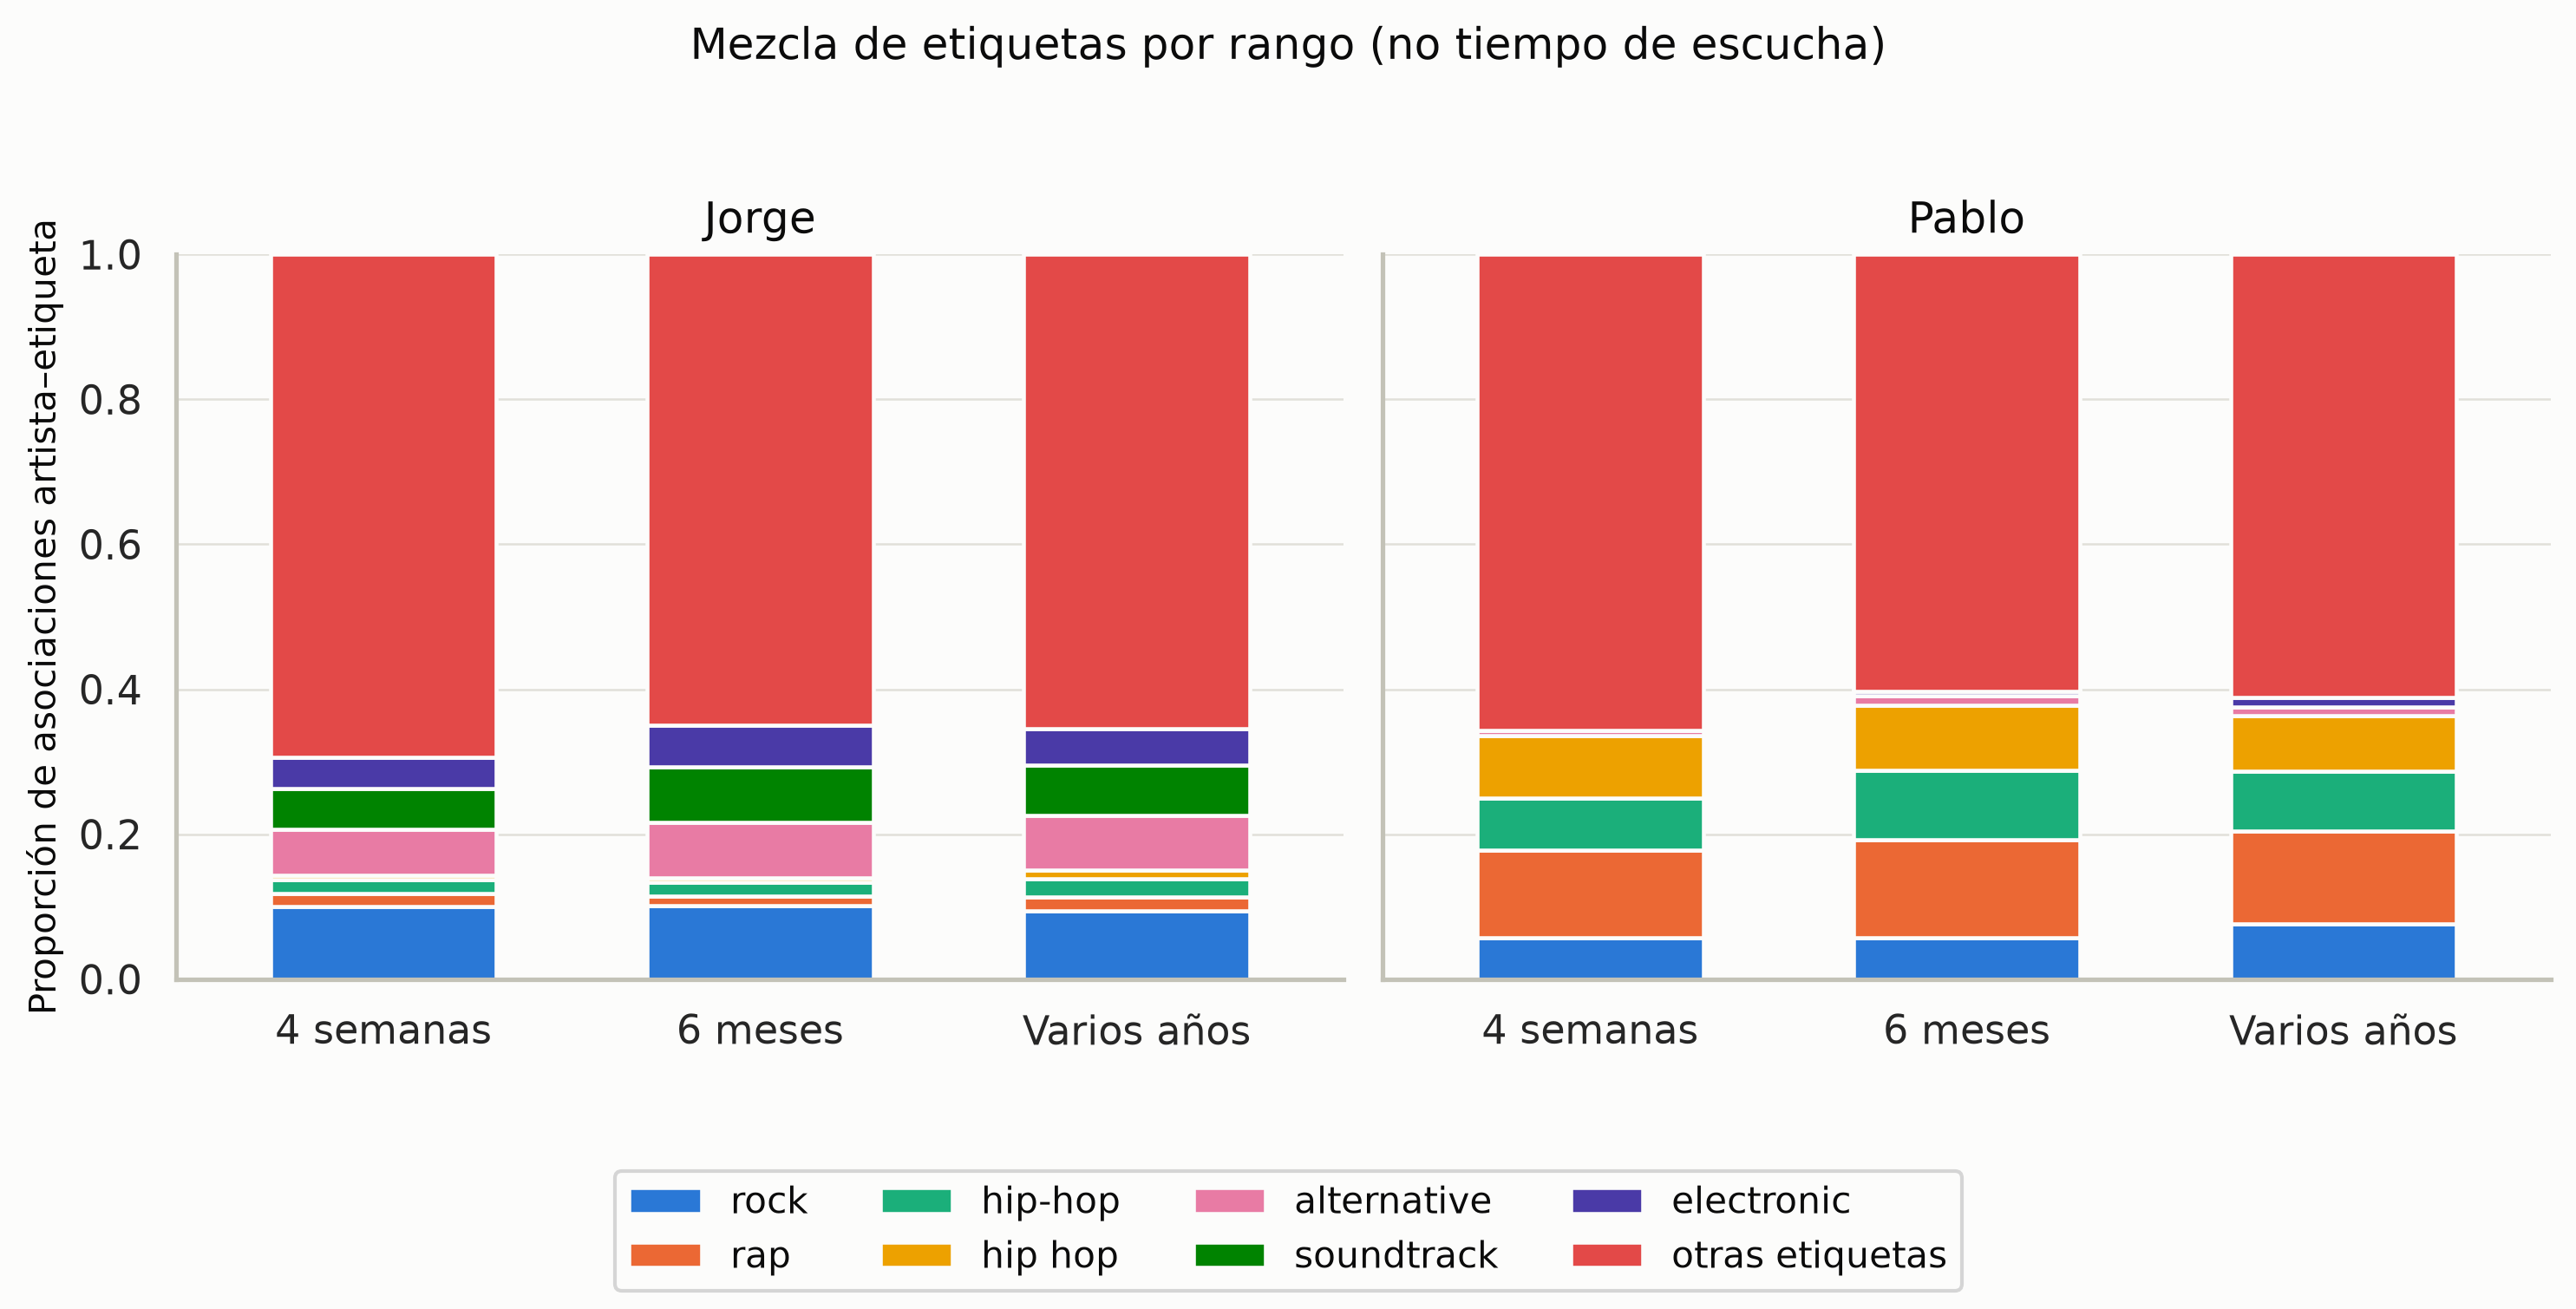
\includegraphics[width=\textwidth]{img/02_generos_por_rango.png}
\caption{Proporciones de asociaciones artista--etiqueta por rango. Las siete etiquetas destacadas y sus colores se mantienen entre paneles; el resto se agrupa. El denominador no es el tiempo de escucha.}
\label{fig:generos-rangos}
\end{figure}

\section{Coincidencia entre ventanas temporales}

Los conjuntos de artistas de cada usuario muestran coincidencias apreciables entre ventanas. Jorge tiene Jaccard de 0,5806 entre cuatro semanas y seis meses, 0,5312 entre cuatro semanas y varios años, y 0,6129 entre seis meses y varios años. Para Pablo son 0,5625, 0,5152 y 0,6667, respectivamente. En ambos casos la mayor coincidencia corresponde a medio y largo plazo.

Los cosenos de etiquetas son aún más elevados: 0,9566--0,9777 en Jorge y 0,9471--0,9717 en Pablo. La composición etiquetada es, por tanto, más parecida que la identidad exacta de los artistas. Hay 31 artistas de Jorge y 34 de Pablo presentes en los tres rangos; 25 y 32, respectivamente, aparecen en uno solo. No se interpreta esta coincidencia como una serie temporal independiente, porque las ventanas se solapan.

\begin{figure}[H]
\centering
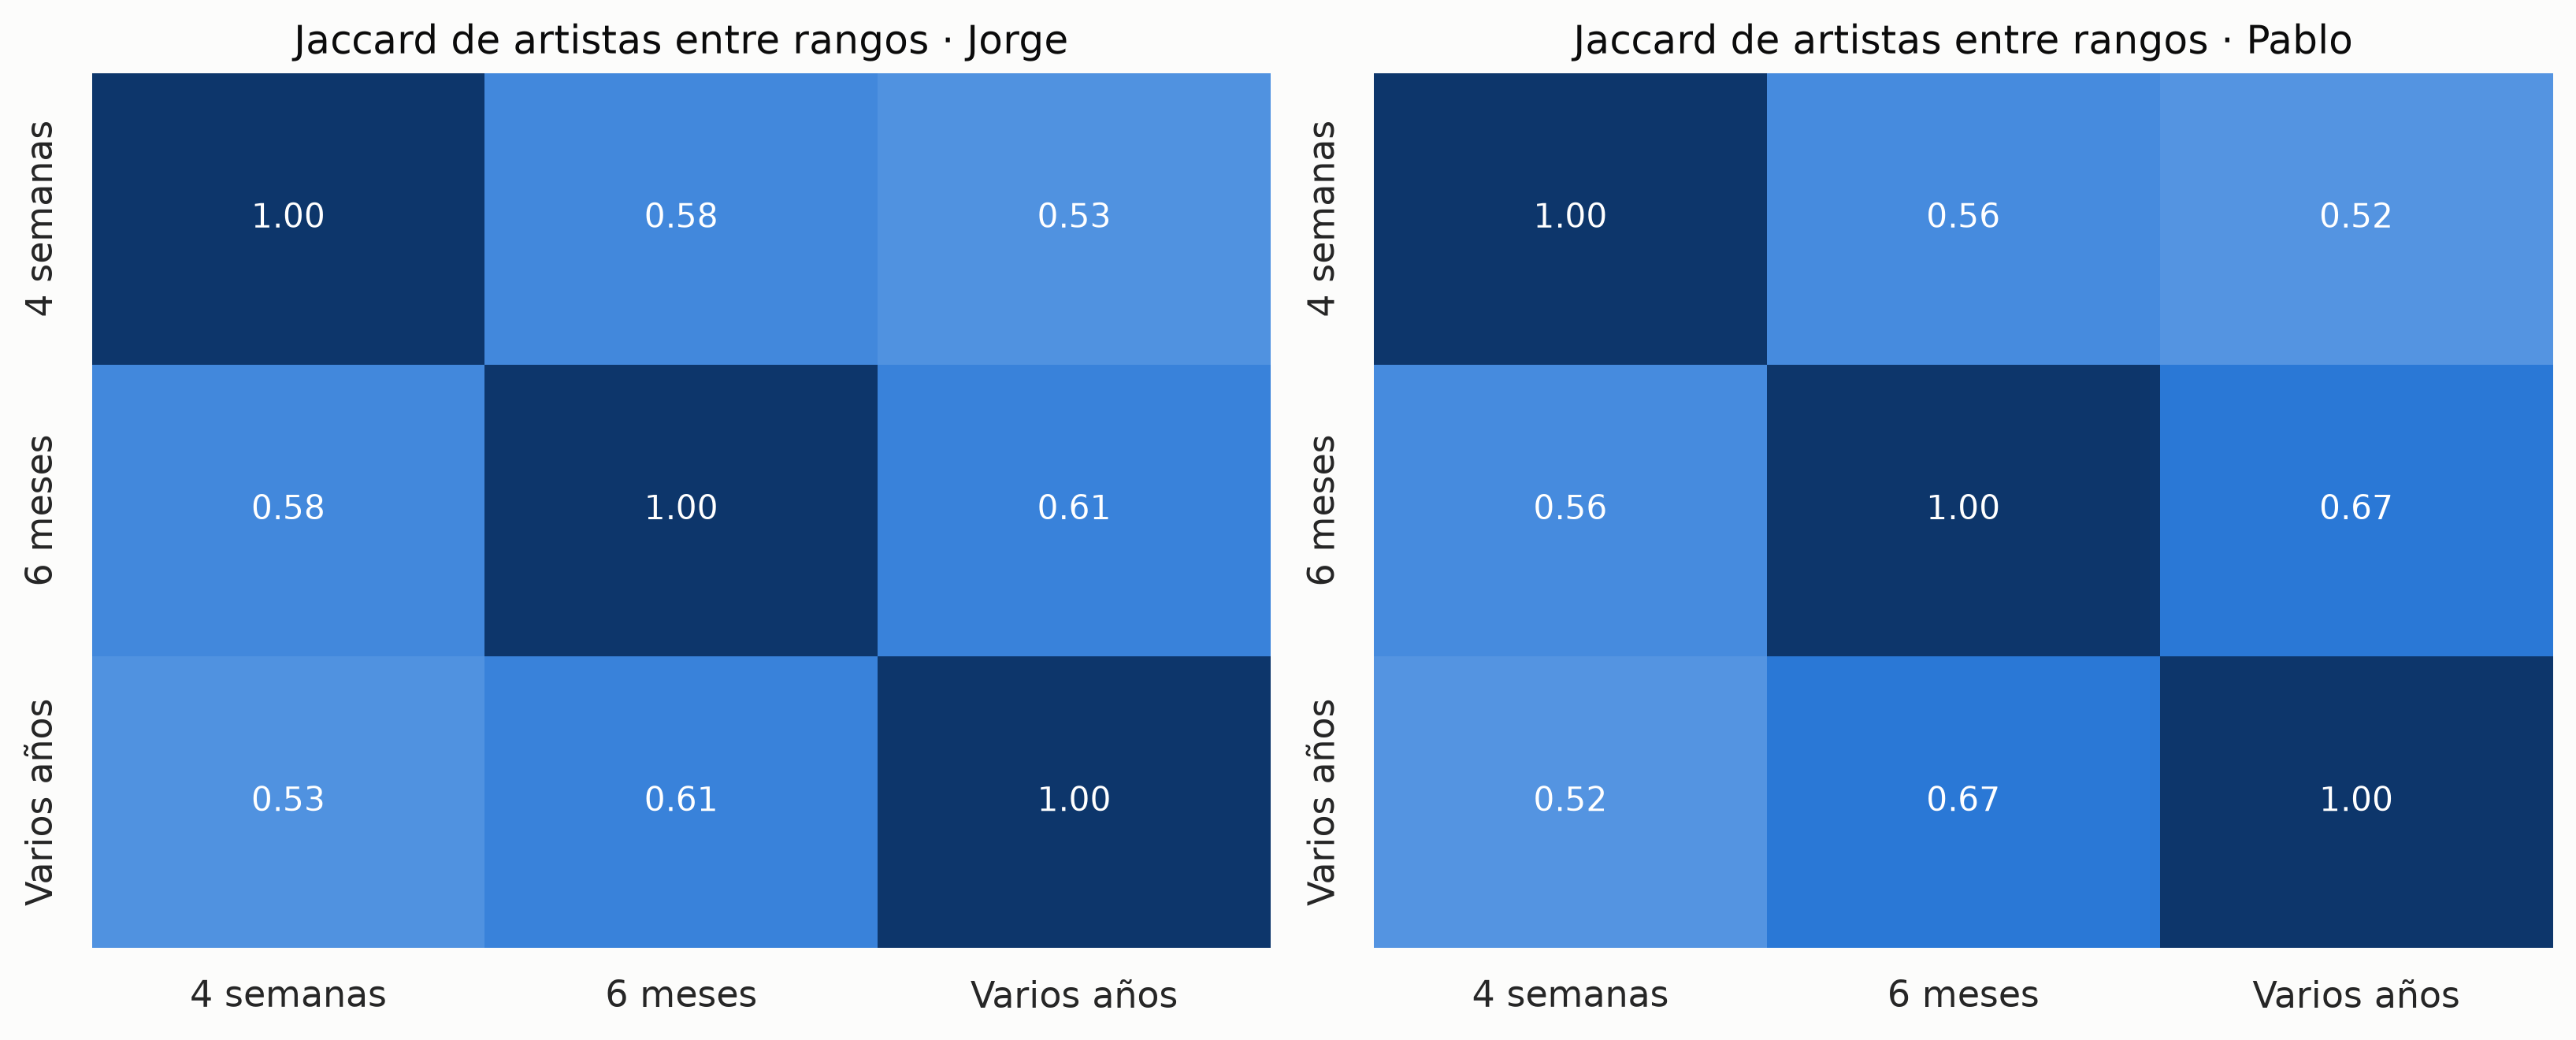
\includegraphics[width=\textwidth]{img/03_estabilidad_rangos.png}
\caption{Jaccard de artistas entre rangos, incluidos los artistas sin etiquetas. La escala común de 0 a 1 y las anotaciones permiten comparar ambas matrices; la diagonal vale 1 por construcción.}
\label{fig:estabilidad}
\end{figure}

\section{Compatibilidad entre usuarios}

La coincidencia global es de \textbf{5 artistas sobre una unión de 140}, de modo que $J=5/140=0{,}0357$. El Jaccard por ventana permanece entre 0,0309 y 0,0417. La similitud del coseno de etiquetas es mayor: 0,3247 en cuatro semanas, 0,3110 en seis meses y 0,4112 en varios años; al reunir las tres ventanas alcanza 0,4686, con 27 etiquetas comunes. No son porcentajes equivalentes de compatibilidad: Jaccard compara identidades y el coseno compara composiciones etiquetadas.

\begin{table}[H]
\centering
\begin{tabular}{lrrr}
\hline
Rango & Artistas comunes & Jaccard & Coseno \\
\hline
4 semanas & 3 & 0,0316 & 0,3247 \\
6 meses & 4 & 0,0417 & 0,3110 \\
Varios años & 3 & 0,0309 & 0,4112 \\
Global & 5 & 0,0357 & 0,4686 \\
\hline
\end{tabular}
\caption{Dos medidas complementarias de coincidencia entre usuarios. Los artistas sin etiquetas se mantienen en el cálculo de Jaccard.}
\label{tab:compatibilidad}
\end{table}

\begin{figure}[H]
\centering
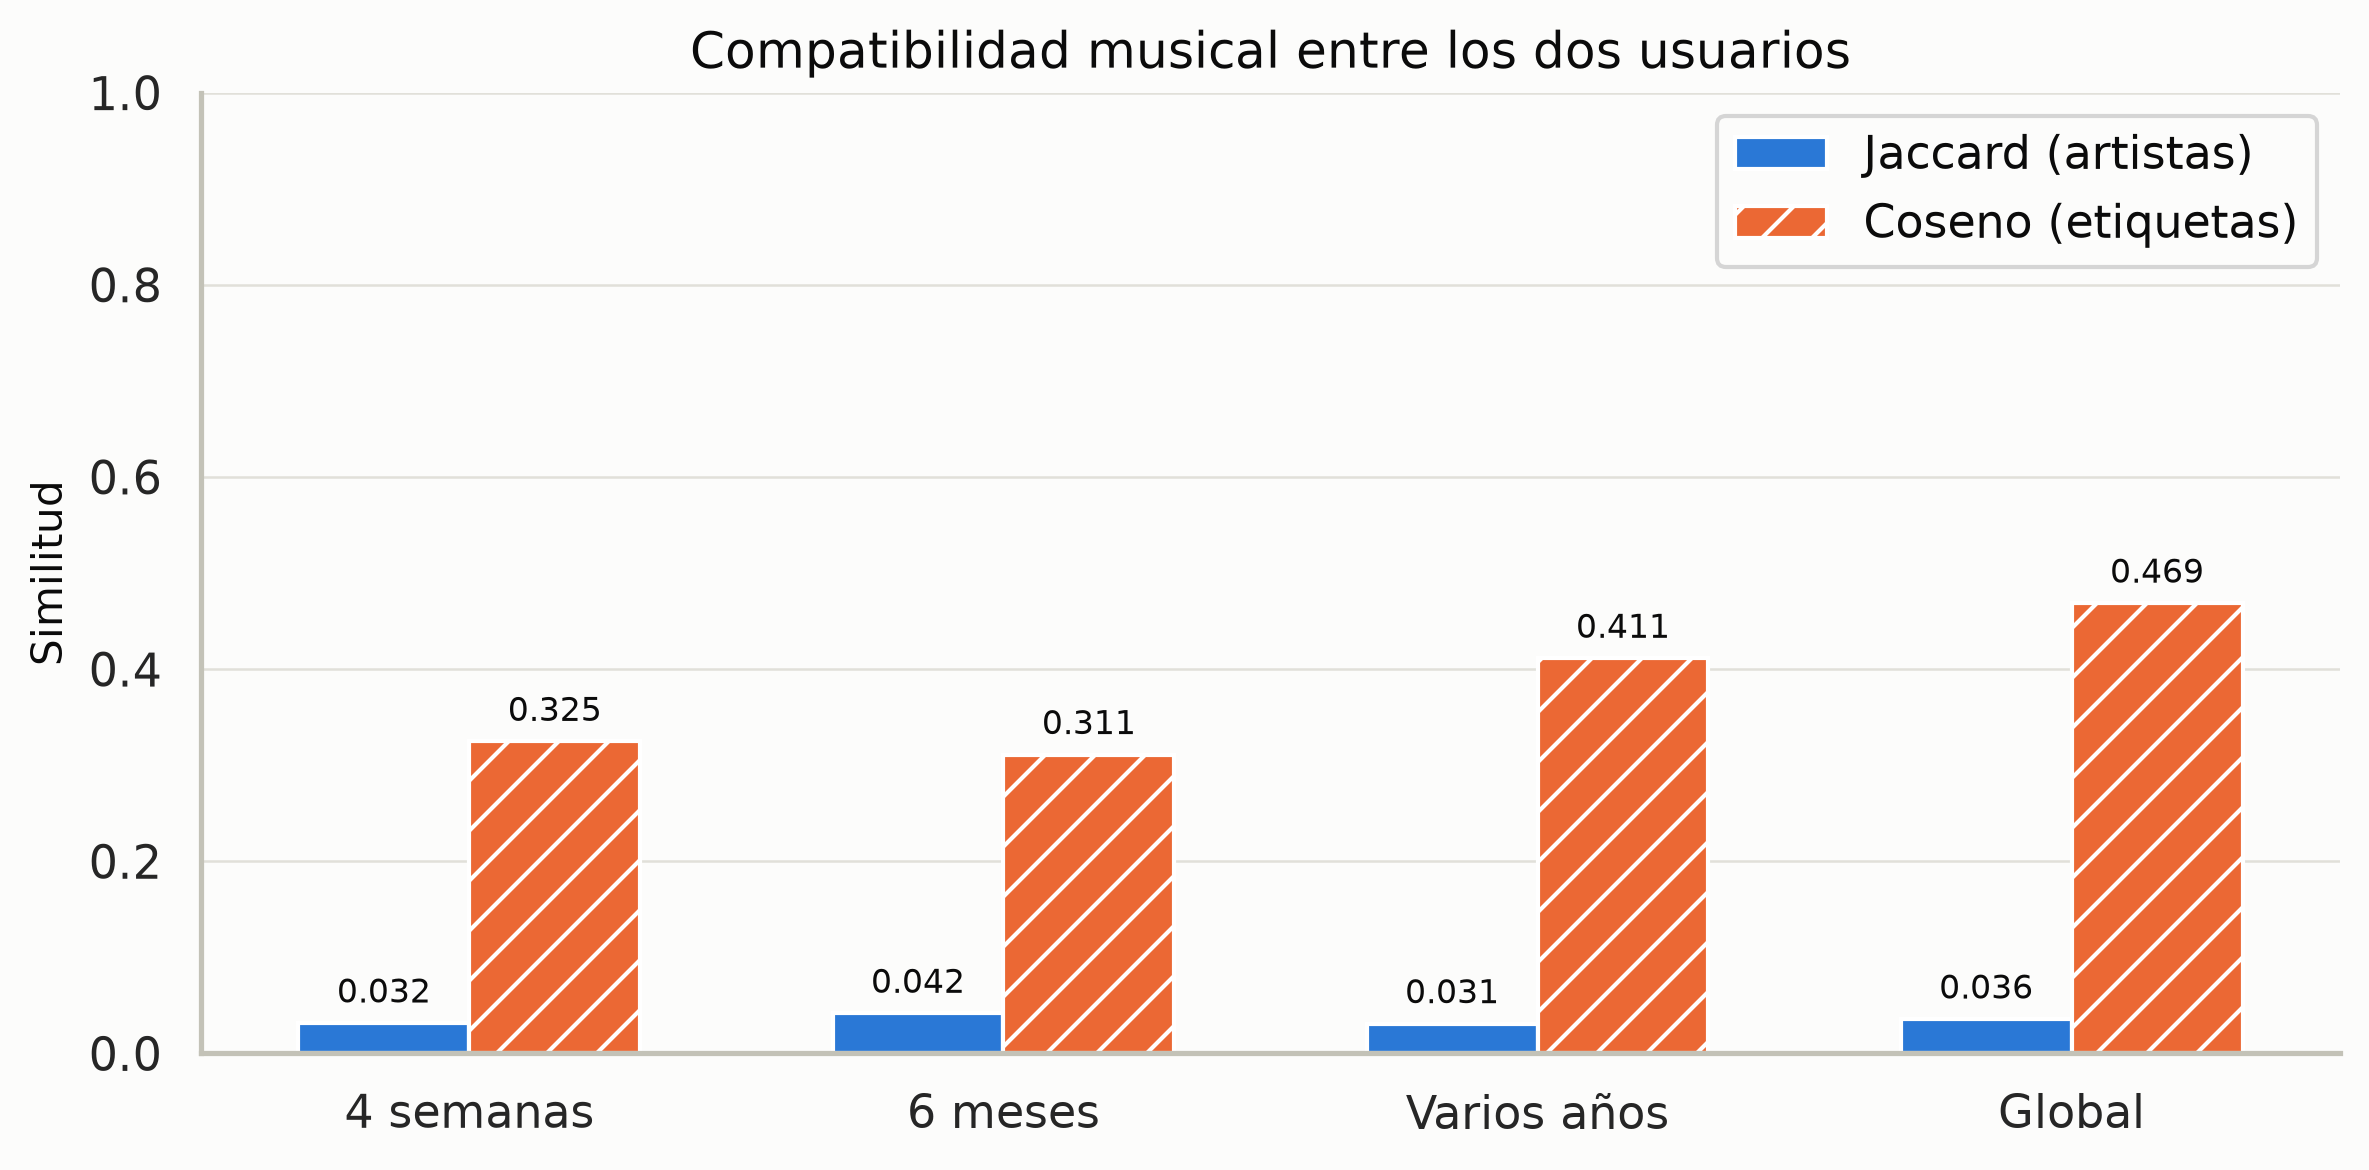
\includegraphics[width=\textwidth]{img/04_compatibilidad.png}
\caption{Jaccard de artistas y coseno de etiquetas por ventana y global. Se conserva una escala común 0--1 y se distinguen las métricas mediante leyenda y trama, además del color.}
\label{fig:compatibilidad}
\end{figure}

El resultado permite afirmar que las listas concretas son muy distintas, pero comparten parte del vocabulario musical, incluido \texttt{rock}. La diferencia entre medidas es coherente con que dos personas escuchen artistas distintos vinculados a etiquetas semejantes. No se transforma el coseno en una valoración personal ni en una probabilidad de compartir gustos.

\section{Cobertura de las fuentes y tratamiento de ausencias}

El enriquecimiento se completó el 4 de noviembre de 2026. Last.fm devuelve oyentes, reproducciones y al menos un vecino para los 140 artistas del historial. Esto no implica cobertura perfecta de todos sus atributos: faltan 20 identificadores MusicBrainz. Deezer aporta fans y número de álbumes para 136 artistas con coincidencia exacta de nombre; los cuatro restantes se mantienen ausentes, sin atribuirles resultados aproximados.

\begin{table}[H]
\centering
\begin{tabular}{lrr}
\hline
Información ausente & Artistas & Porcentaje \\
\hline
Etiquetas del CSV & 5 & 3,57\% \\
Oyentes Last.fm & 0 & 0,00\% \\
Reproducciones Last.fm & 0 & 0,00\% \\
Identificador MusicBrainz & 20 & 14,29\% \\
Sin vecinos similares & 0 & 0,00\% \\
Fans Deezer & 4 & 2,86\% \\
Álbumes Deezer & 4 & 2,86\% \\
\hline
\end{tabular}
\caption{Ausencias sobre los 140 artistas únicos. Los campos no son excluyentes: un artista puede carecer de varios atributos.}
\label{tab:cobertura-resultados}
\end{table}

\begin{figure}[H]
\centering
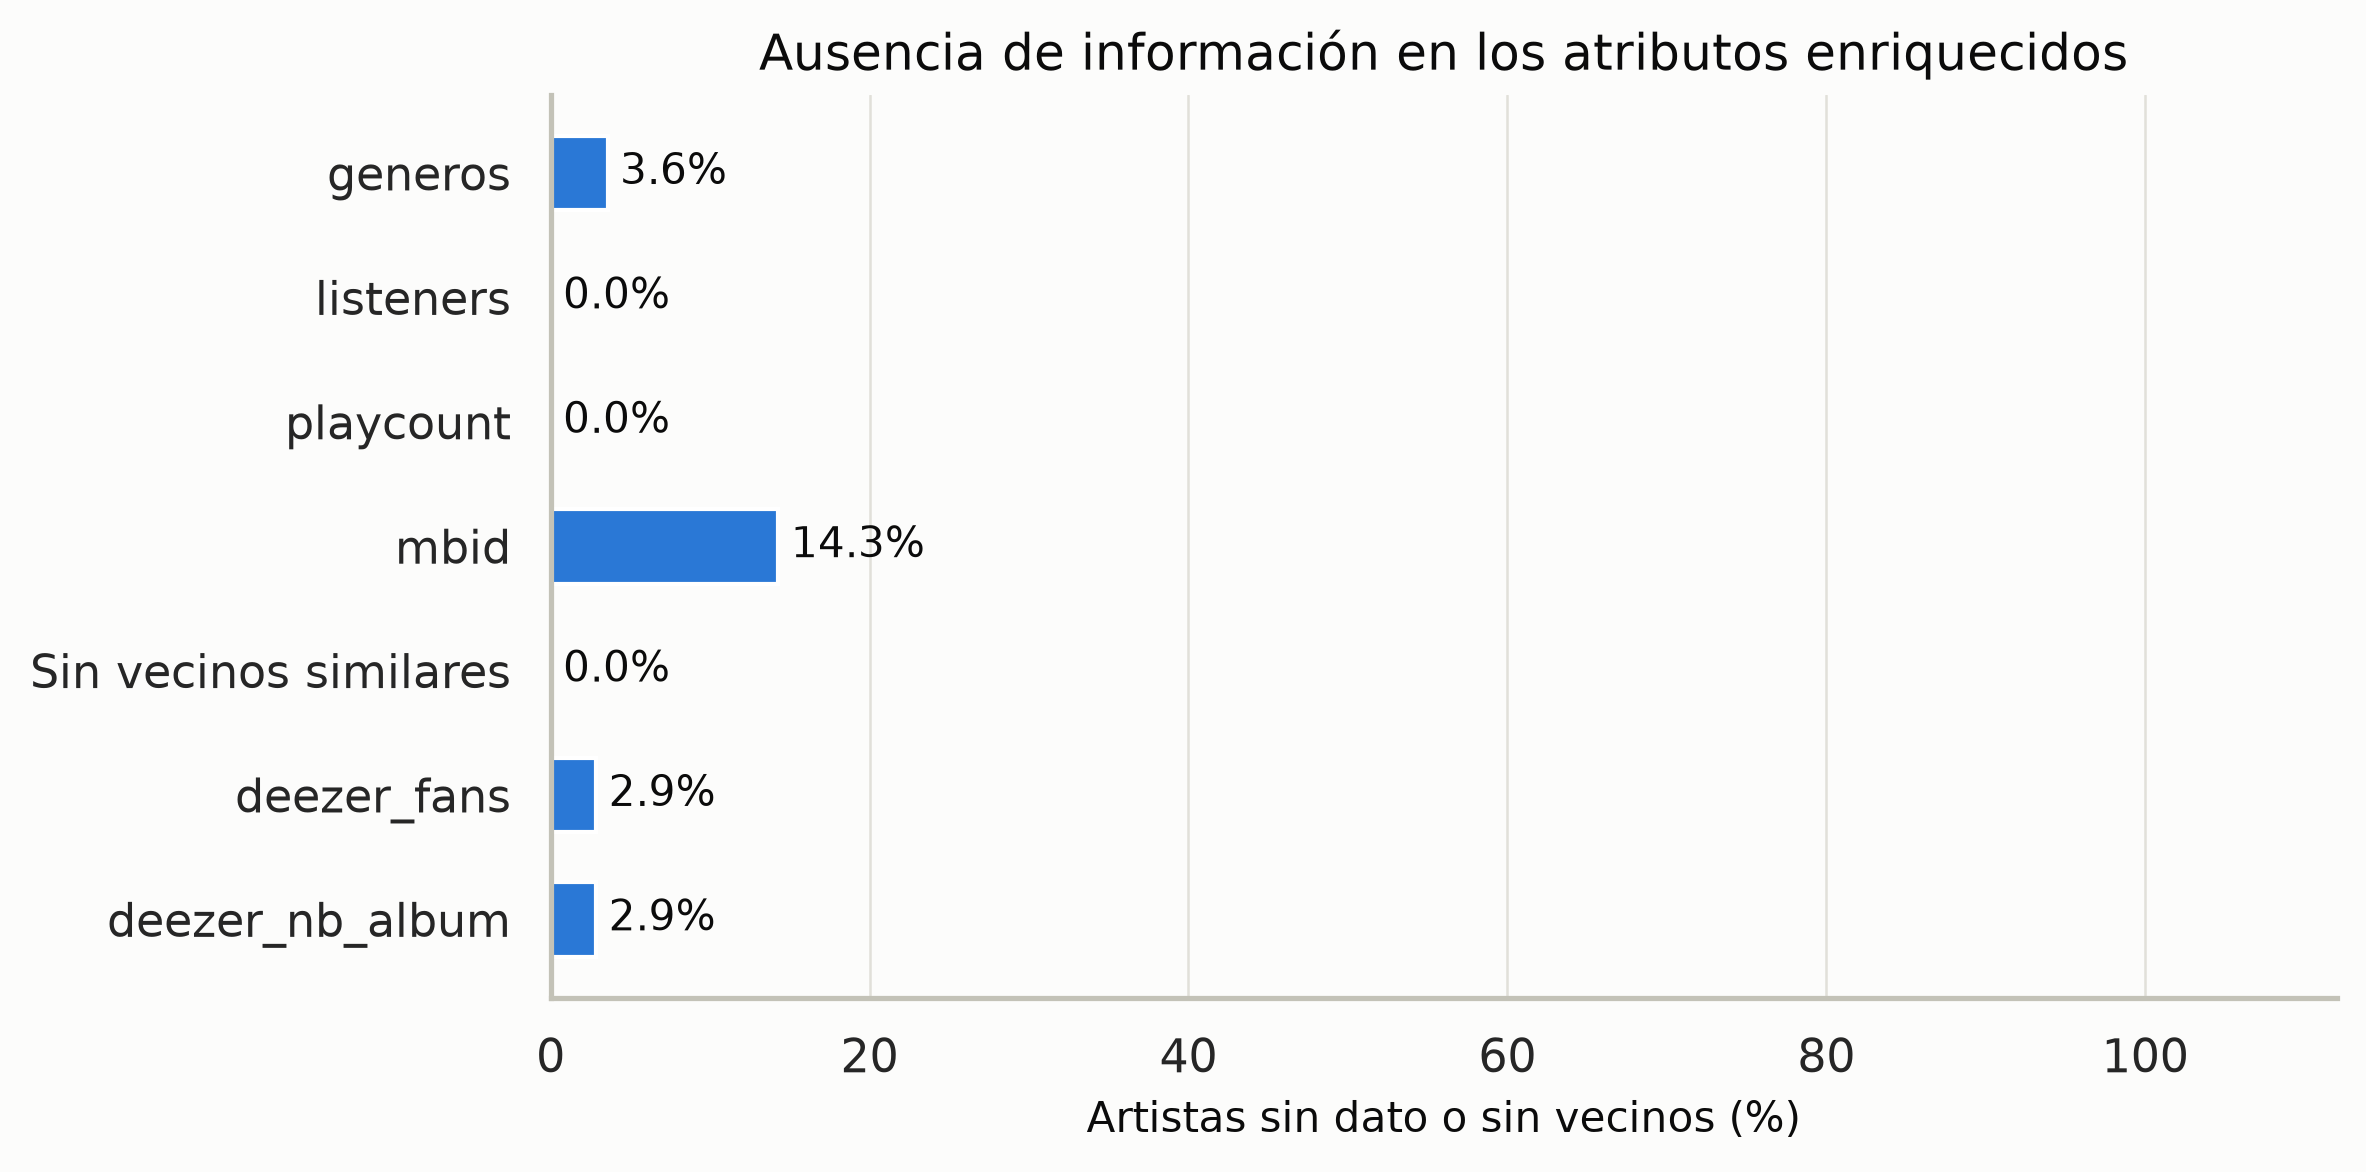
\includegraphics[width=\textwidth]{img/09_nulos.png}
\caption{Porcentaje sin información por atributo. Las barras parten de cero y tienen una escala porcentual común; ``sin vecinos'' cuenta listas vacías, no solo nulos de almacenamiento.}
\label{fig:nulos}
\end{figure}

El procedimiento de imputación no modifica ningún valor de oyentes o reproducciones, porque están completos. Genera cuatro valores de fans en una columna separada, según las reglas de mediana descritas en el Capítulo~\ref{chap:modelo}; la mediana global observada de fans es 16\,042,5. Las columnas originales y las banderas de imputación se conservan. Los análisis siguientes usan observaciones reales: la correlación entre fuentes tiene 136 casos, no 140.

\section{Popularidad externa y posición personal}

\begin{table}[H]
\centering
\begin{tabular}{llrrr}
\hline
Usuario & Rango & $n$ & Spearman $\rho$ & Valor $p$ \\
\hline
Jorge & 4 semanas & 48 & 0,1845 & 0,2092 \\
Jorge & 6 meses & 50 & $-0{,}0033$ & 0,9818 \\
Jorge & Varios años & 50 & $-0{,}0337$ & 0,8165 \\
Pablo & 4 semanas & 50 & $-0{,}1055$ & 0,4659 \\
Pablo & 6 meses & 50 & 0,2548 & 0,0741 \\
Pablo & Varios años & 50 & 0,3275 & 0,0202 \\
\hline
\end{tabular}
\caption{Correlación entre posición numérica y logaritmo de oyentes de Last.fm, solo con casos observados. Los valores $p$ son exploratorios y no están corregidos por las seis comparaciones.}
\label{tab:popularidad}
\end{table}

No aparece una asociación de igual signo y magnitud en los seis perfiles. La mayor correlación es la de Pablo en varios años ($\rho=0{,}3275$): al aumentar la posición numérica, es decir, al bajar en el ranking, tiende a aumentar la popularidad externa. No significa que los artistas más populares estén mejor situados, sino lo contrario. Su valor $p$ sin ajustar es 0,0202, pero se han examinado seis combinaciones y no existe un diseño confirmatorio; tampoco las ventanas son independientes. El resultado se describe como una asociación moderada y localizada, sin generalizar una preferencia estable o causal.

\begin{figure}[H]
\centering
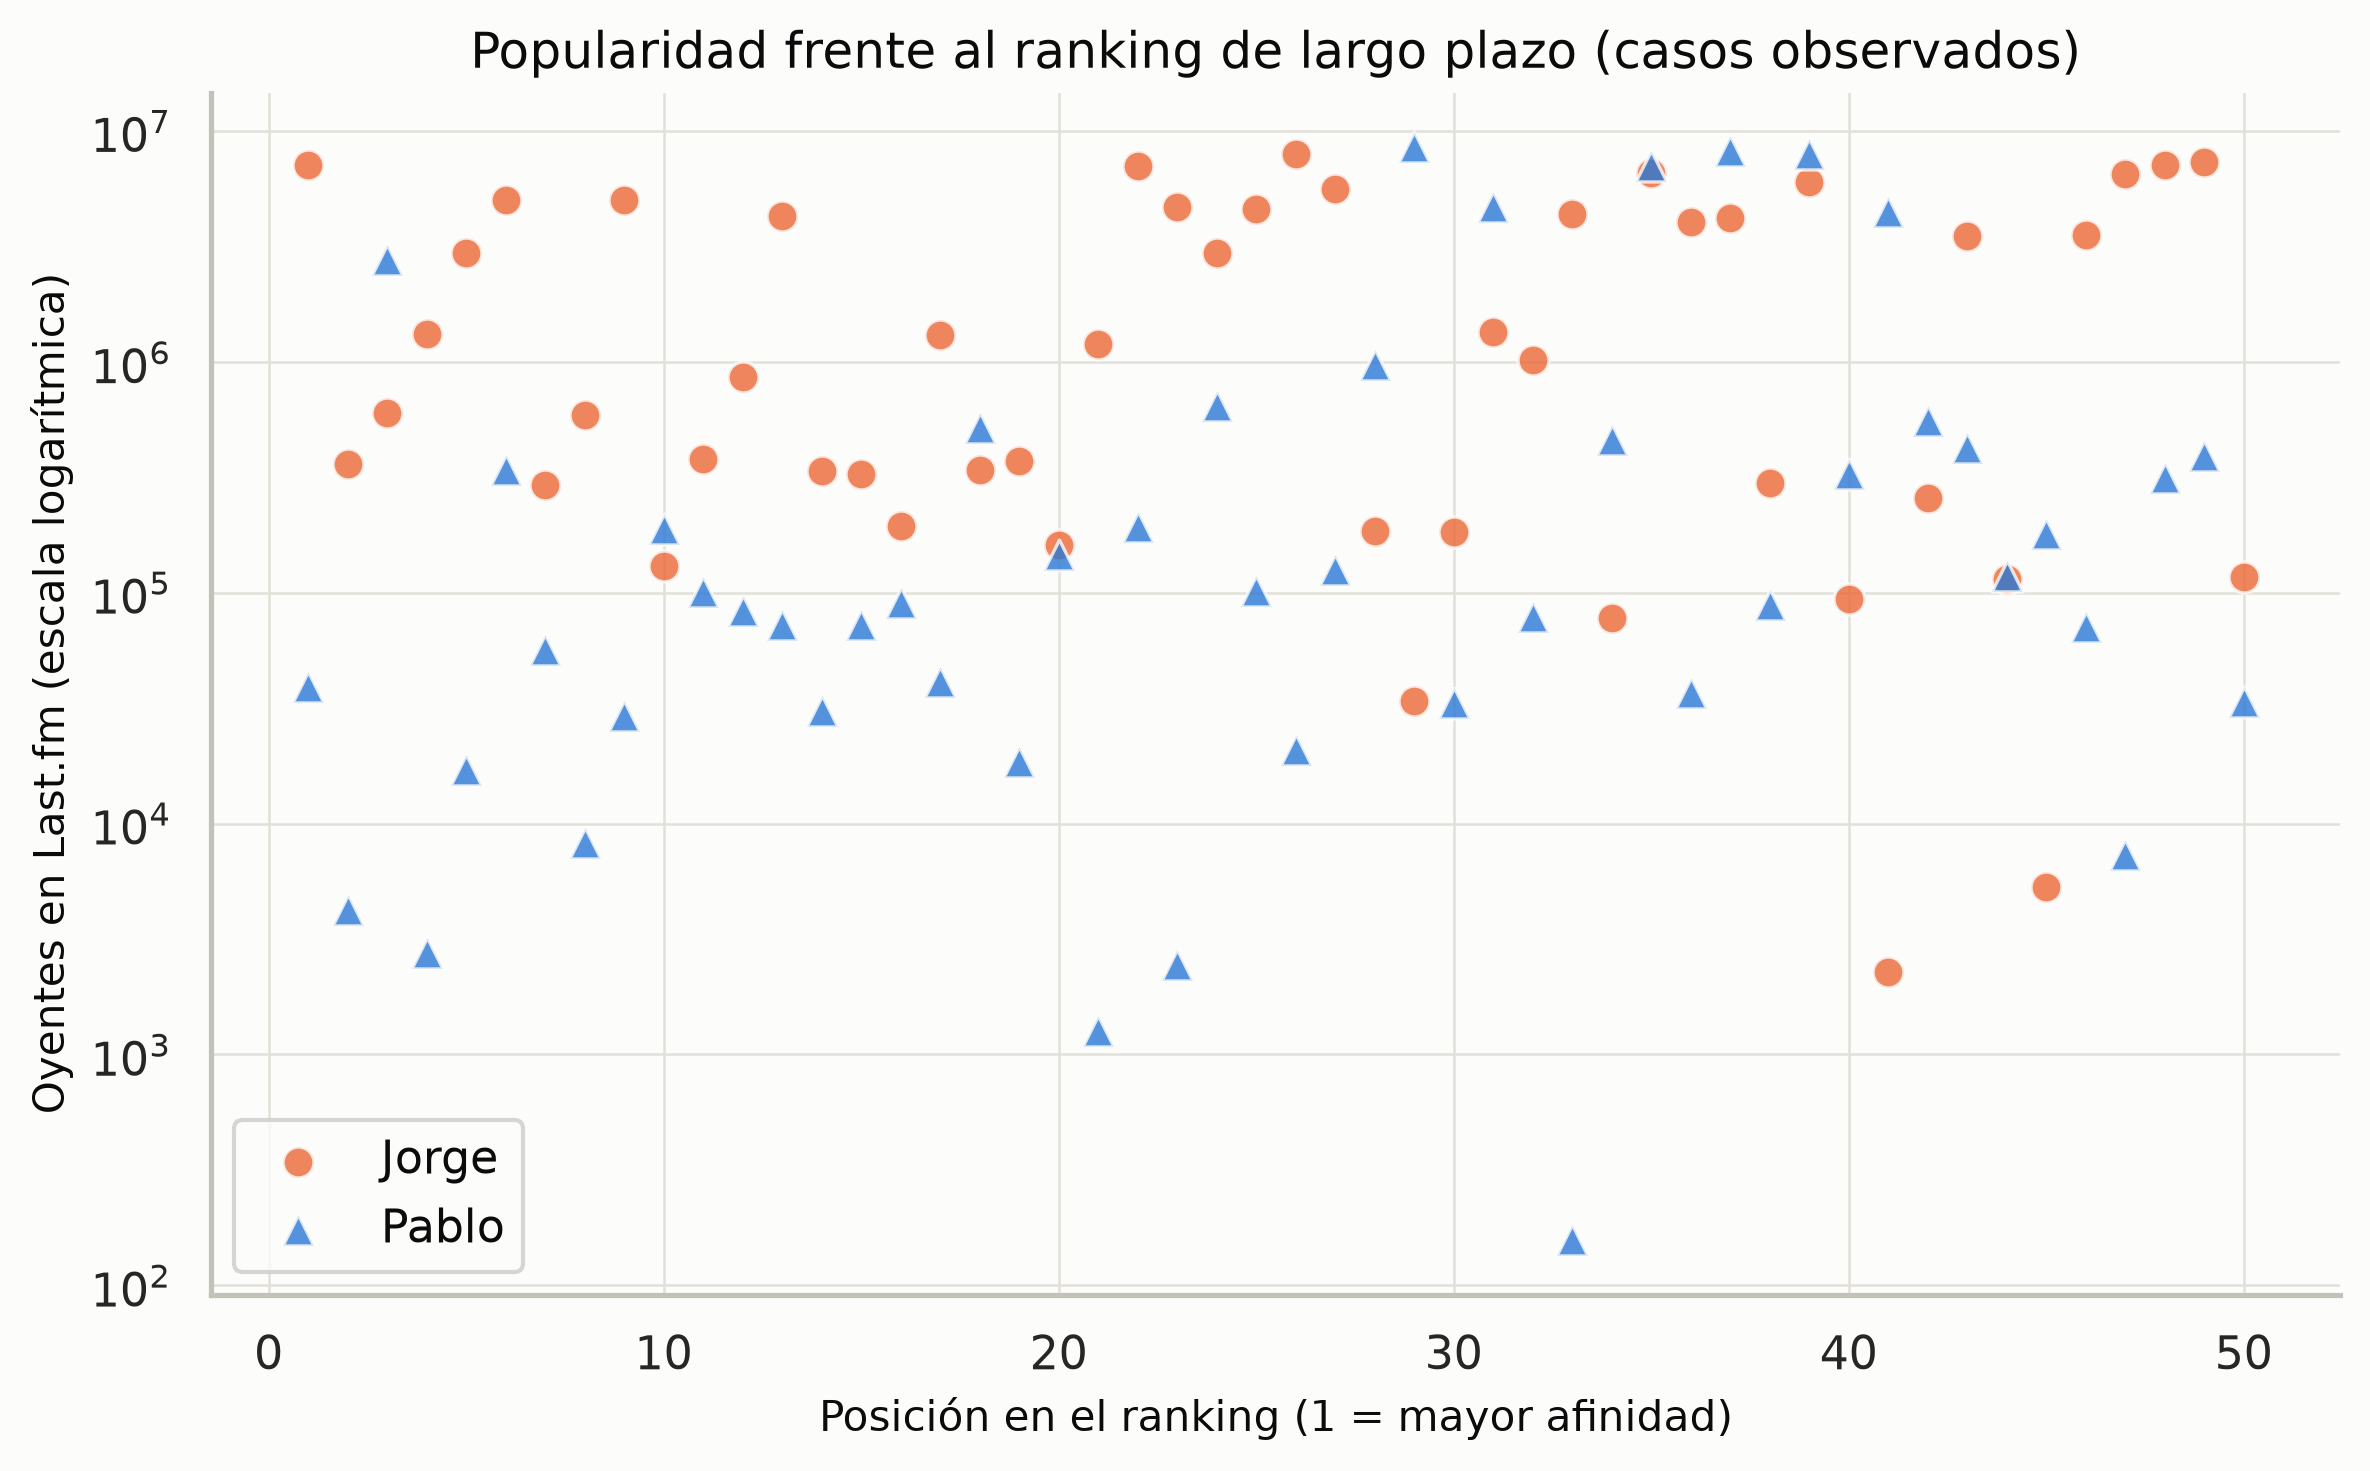
\includegraphics[width=\textwidth]{img/05_popularidad_rank.png}
\caption{Oyentes externos frente a posición personal en la ventana larga. La escala logarítmica permite representar varios órdenes de magnitud; usuario y forma de los puntos se mantienen identificados en la leyenda. Cada punto es una entrada del ranking, no una reproducción.}
\label{fig:popularidad}
\end{figure}

Entre las dos medidas externas de popularidad, oyentes de Last.fm y fans de Deezer, se obtiene $\rho=0{,}6830$ con 136 pares observados ($p\simeq5{,}19\times10^{-20}$). La relación positiva indica ordenaciones parcialmente concordantes dentro del conjunto seleccionado, pero no intercambiabilidad: son plataformas y acciones de usuario distintas. No se utiliza esta asociación para rellenar los cuatro fans ausentes ni se presenta como representativa de todos los artistas de ambas plataformas.

\section{Afinidad de candidatos nuevos}

Se generan 20 candidatos fuera de los dos historiales y se consultan sus propios vecinos. Los \textbf{20 son puntuables para ambos usuarios}; esta cobertura se refiere a la disponibilidad del cálculo, no a que encajen con ambos perfiles. De hecho, \textbf{ninguno de los veinte obtiene puntuación positiva para los dos usuarios a la vez}. Cada uno presenta solapamiento ponderado con un perfil y cero con el otro.

La Figura~\ref{fig:afinidad} muestra diez candidatos ordenados por la media de sus dos puntuaciones, con identificadores anónimos. El candidato C01 obtiene 0,2175 en Jorge y 0 en Pablo; C02 obtiene 0 y 0,2156, respectivamente. Sus medias, 0,1087 y 0,1078, no representan una afinidad compartida. La media prioriza una puntuación unilateral relativamente alta, de modo que no debe interpretarse este top como una selección de consenso. Un cero significa ausencia de vecinos coincidentes en el historial truncado, no rechazo declarado del artista.

\begin{figure}[H]
\centering
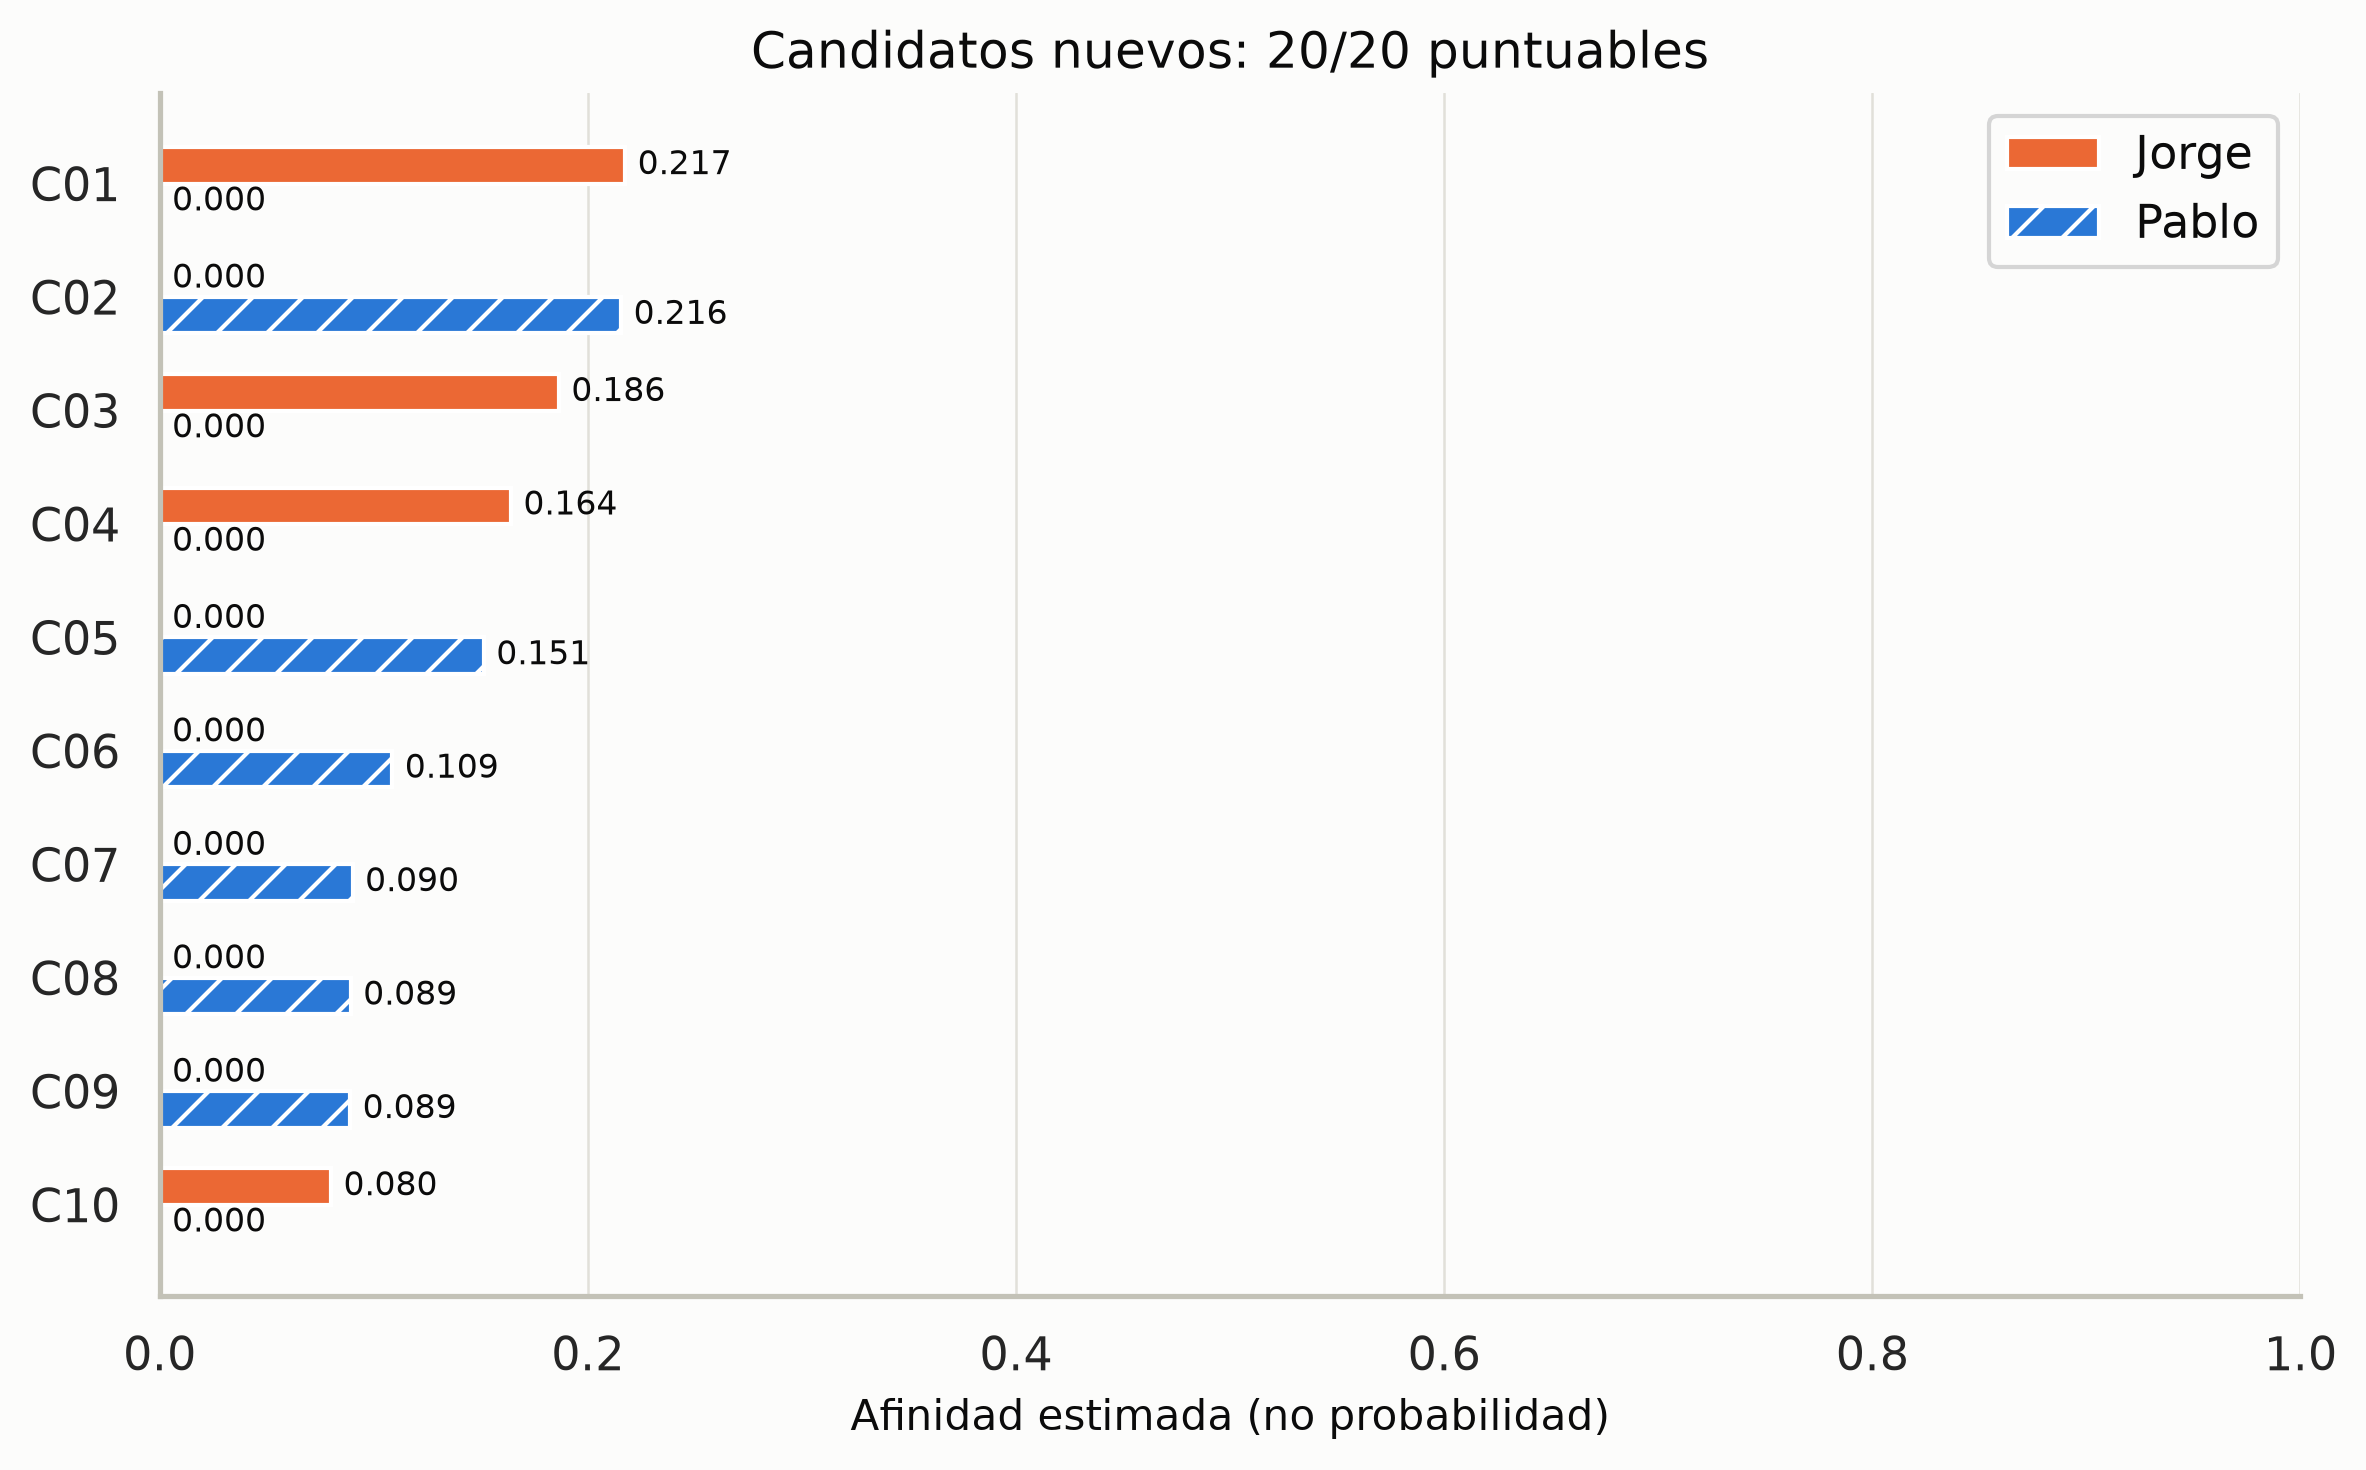
\includegraphics[width=\textwidth]{img/06_afinidad.png}
\caption{Diez candidatos anónimos con mayor afinidad media. El eje común 0--1, las etiquetas numéricas y la trama permiten ver tanto las diferencias como los ceros. La cobertura 20/20 indica que el cálculo está disponible, no una tasa de acierto.}
\label{fig:afinidad}
\end{figure}

\begin{table}[H]
\centering
\small
\begin{tabular}{lrrrrr}
\hline
Usuario & Ocultos & Controles & Mediana ocultos & Mediana controles & Valor $p$ \\
\hline
Jorge & 10 & 20 & 0,1069 & 0,0435 & 0,0801 \\
Pablo & 10 & 20 & 0,1647 & 0,0000 & 0,000205 \\
\hline
\end{tabular}
\caption{Comprobación exploratoria \emph{leave-one-out}. El valor $p$ corresponde a la prueba U unilateral (ocultos mayores que controles); los controles no son ejemplos negativos ni una muestra independiente.}
\label{tab:loo}
\end{table}

Las medianas de los favoritos ocultos son mayores que las de los candidatos-control en ambos usuarios. Los estadísticos U son 132,0 en Jorge y 177,5 en Pablo. Esta comparación muestra el comportamiento interno de la heurística, pero no proporciona precisión, tasa de acierto ni garantía de que gusten las recomendaciones: candidatos y favoritos comparten el mecanismo de selección y no se dispone de valoraciones independientes.

\section{Agrupamiento exploratorio}
\label{sec:resultados-clustering}

De los 140 artistas, cinco carecen de etiquetas y otros dos quedan sin ninguna tras exigir soporte mínimo de dos artistas por etiqueta. La matriz final tiene \textbf{133 artistas y 52 etiquetas}; se descartan 78 etiquetas de soporte uno. Esta selección limita la representación de estilos raros y debe tenerse en cuenta al interpretar los grupos.

\begin{figure}[H]
\centering
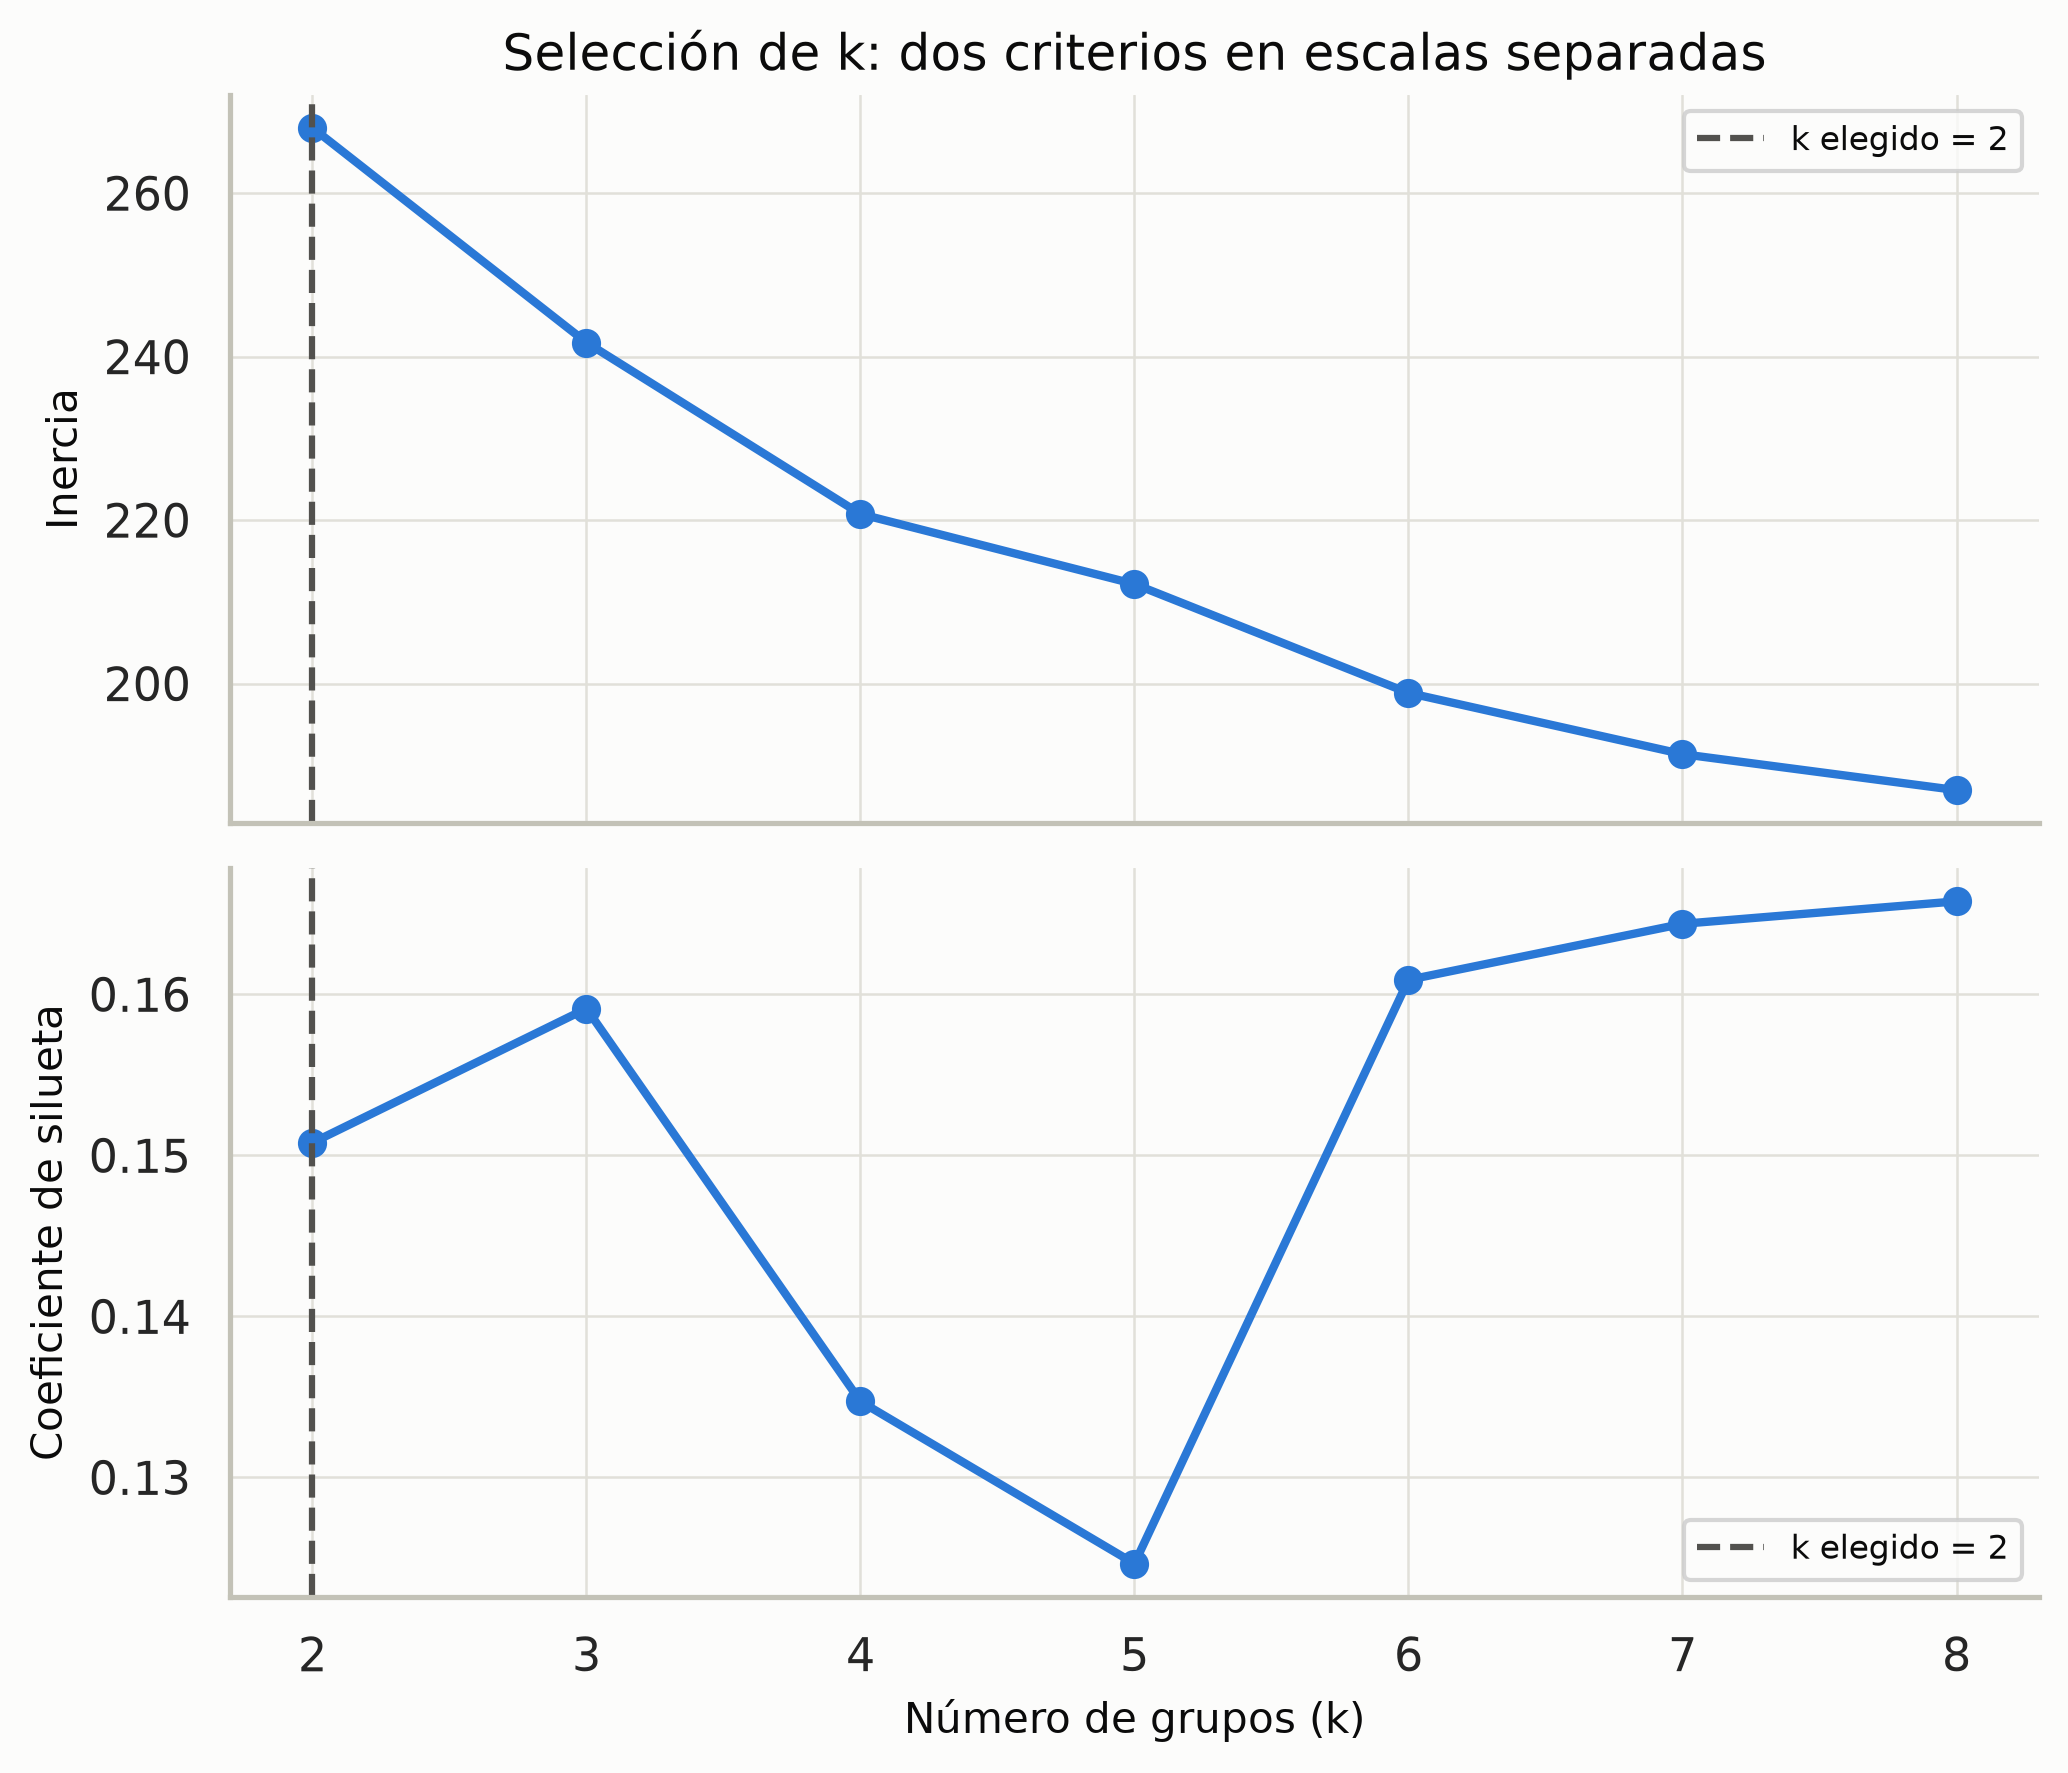
\includegraphics[width=0.86\textwidth]{img/08_seleccion_k.png}
\caption{Inercia y silueta para $k=2,\ldots,8$, en paneles con escalas independientes. La inercia disminuye al aumentar el número de grupos, pero no constituye por sí sola una mejora de interpretación.}
\label{fig:seleccion-k}
\end{figure}

La mejor silueta observada es 0,1658 con $k=8$. La regla predefinida elige el menor $k$ cuya silueta queda a menos de 0,02 del máximo: resulta \textbf{$k=2$}, con silueta 0,1508 e inercia 267,9952. La silueta es baja en todos los casos, por lo que la separación no es fuerte. La elección prioriza una descripción sencilla; no demuestra que existan exactamente dos familias musicales naturales.

El grupo 0 contiene 28 artistas y se caracteriza, por sobrerrepresentación respecto al conjunto, mediante \texttt{spanish hip-hop}, \texttt{rap} y \texttt{spanish rap}. El grupo 1 contiene 105 artistas y sus etiquetas de mayor sobrerrepresentación son \texttt{80s}, \texttt{alternative} y \texttt{alternative metal}; su mayor tamaño y heterogeneidad impiden resumirlo como un único género. Las etiquetas del perfil se eligen por cociente de prevalencias (\emph{lift}), no por frecuencia absoluta dentro del grupo.

\begin{table}[H]
\centering
\begin{tabular}{lrrr}
\hline
Grupo & Artistas únicos & Presentes en Jorge & Presentes en Pablo \\
\hline
0 & 28 & 5 & 24 \\
1 & 105 & 64 & 45 \\
\hline
\end{tabular}
\caption{Pertenencia de los artistas agrupados a los rankings de cada usuario. Un artista compartido cuenta en ambas columnas, por lo que estas no suman el total de artistas únicos.}
\label{tab:clusters-usuarios}
\end{table}

\begin{figure}[H]
\centering
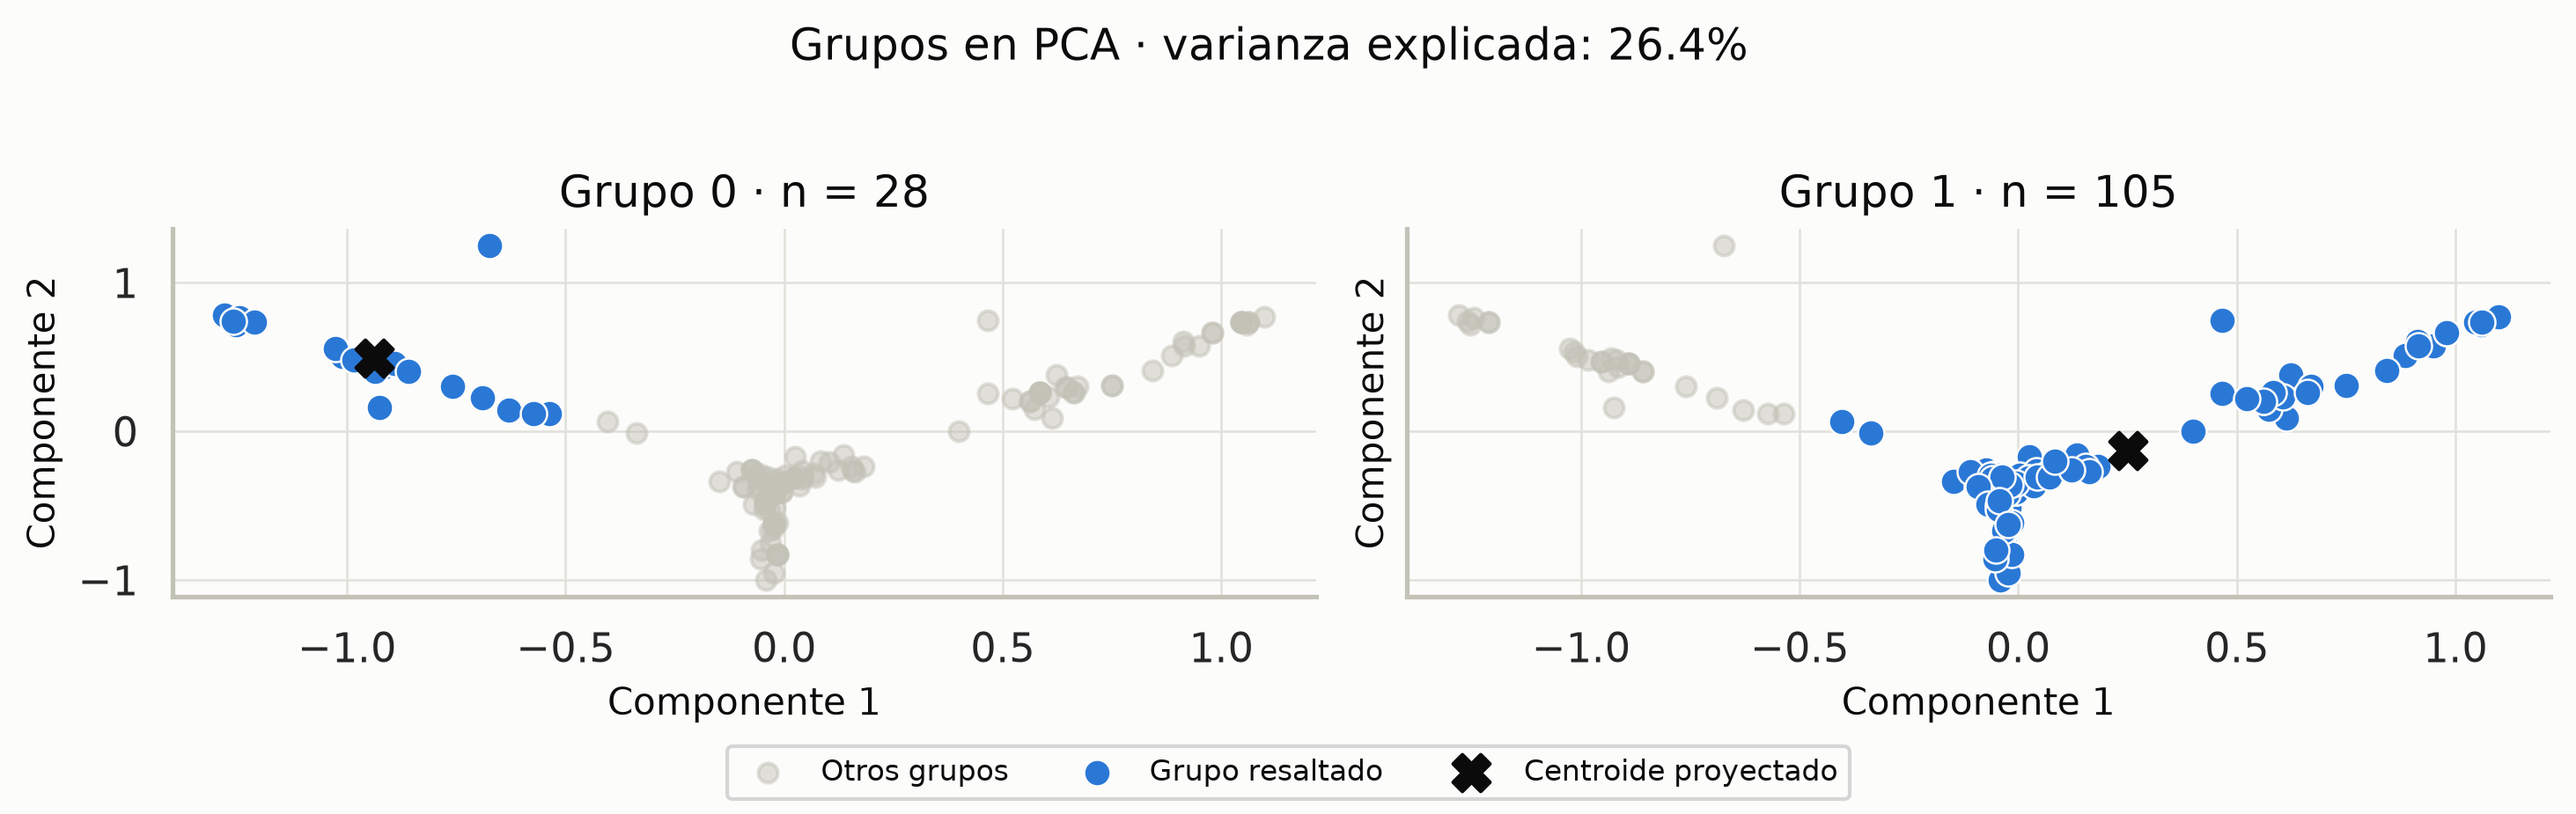
\includegraphics[width=\textwidth]{img/07_clustering_pca.png}
\caption{Proyección PCA con un panel por grupo. El azul destaca el grupo y el gris da contexto; la cruz representa su centroide proyectado. El ajuste de K-Means se realiza en las 52 dimensiones originales, no en este plano.}
\label{fig:pca}
\end{figure}

Las dos primeras componentes explican el \textbf{26,42\%} de la varianza. La proyección pierde casi tres cuartas partes de la variación: ni la proximidad ni la separación visual en dos dimensiones bastan para validar el agrupamiento. El grupo orientado al rap reúne una fracción mayor del perfil de Pablo (24 de sus 69 artistas agrupados) que del de Jorge (5 de 69), en consonancia con las frecuencias de etiquetas, sin constituir una prueba independiente de ellas.

\begin{figure}[H]
\centering
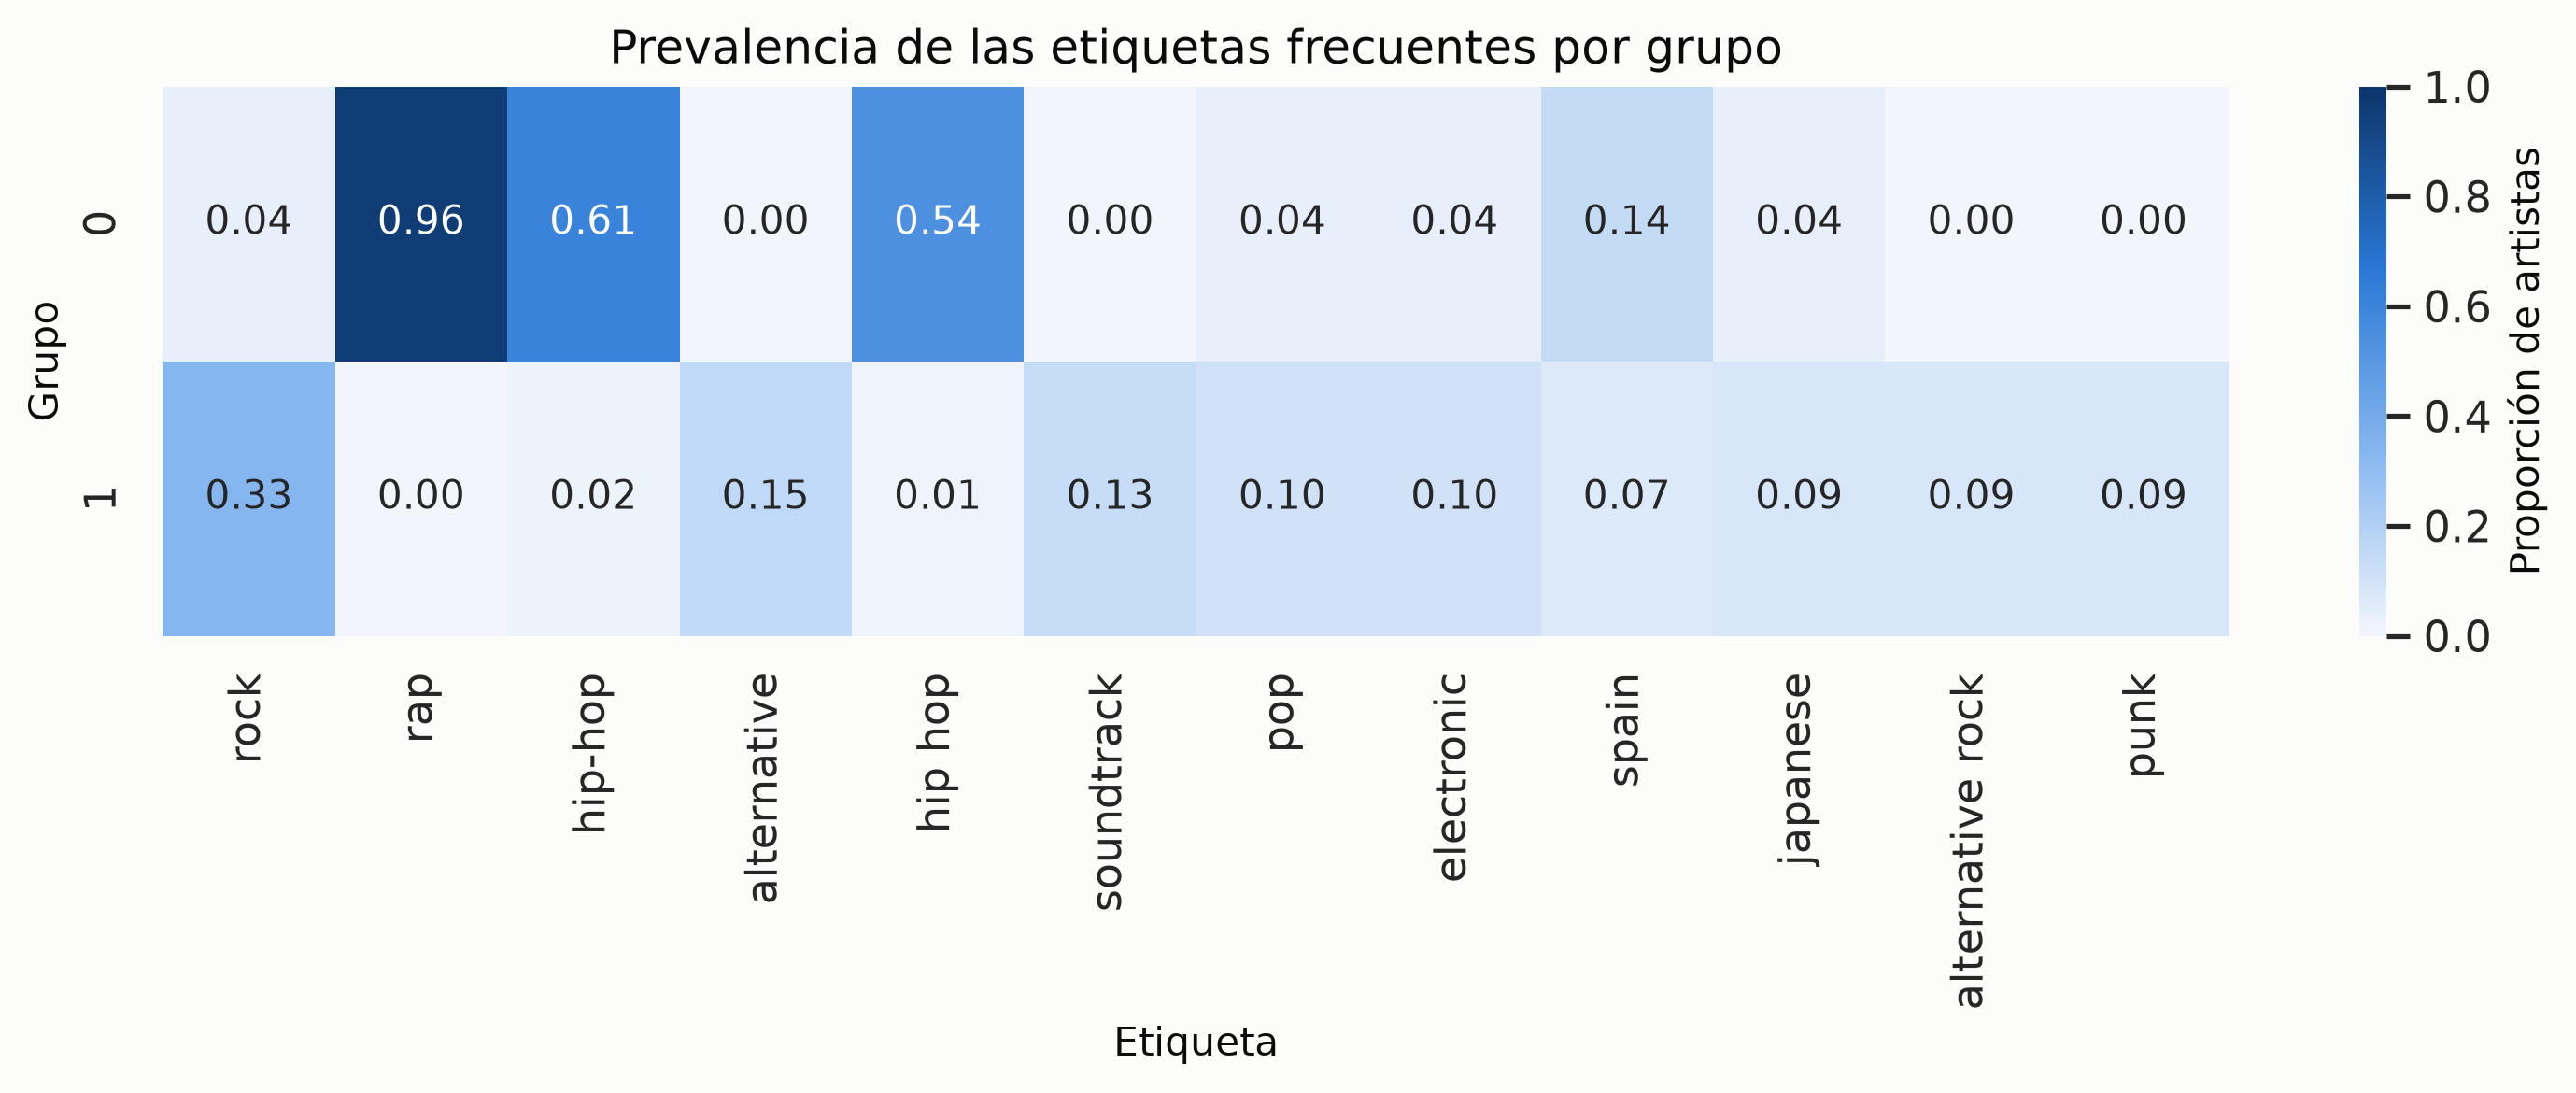
\includegraphics[width=\textwidth]{img/07b_perfil_clusters.png}
\caption{Prevalencia interna de las doce etiquetas más frecuentes de la matriz. La escala secuencial común representa proporciones entre 0 y 1; esta vista complementa las etiquetas elegidas por \emph{lift}.}
\label{fig:perfil-clusters}
\end{figure}
